\section{Einleitung}

Im Zuge der Blockveranstaltung II2008 Physical Computing wurde ein sensorgesteuertes Modellauto entwickelt, welches einer weißen Linie auf schwarzer Fahrbahn folgen muss. Als zentrale Steuereinheit wurde ein ESP32 verwendet, der Antrieb, Lenkung und Sensorik vereint. Die Basis des Modellautos stellt der 2WD RC Smart Chassis Bausatz. Darin enthalten sind ein DC-Motor, der das Fahrzeug antreibt und ein Servo-Motor, der die Lenkachse bewegt. Zur Erkennung der Linie wird ein QRTX-Reflectance Sensor verwendet, der mittels 16 Infrarot-LEDs und Photoresistoren, die in einer Reihe angeordnet sind, arbeitet. Aufgeteilt in zwei Teams wurden 2 verschiedene Autos aus dieser Grundkonfiguration entwickelt, die sich äußerlich sehr ähnlich sehen, sich jedoch gerade bei dem Ansteuern des Reflexionssensor stark unterscheiden. Diese Dokumentation soll einen Einblick in den Entwicklungsprozess eines dieser Modellautos vermitteln. Ziel ist es, durch Folgen eines einfachen Kurses die Grundlage für die Weiterentwicklung zu schaffen. Das Regelwerk der MCU-Rally, an der dieses Fahrzeug einmal antreten soll, schreibt den Einsatz eines Renesas Microcontroller vor, der mit dem ESP32 Chip seriell kommuniziert. Dadurch ist ein Interface zur Kontrolle nötig.

\section{Entwicklung eines MCU-Rally Cars}

	\subsection{Aufbau der Komponenten}
    
    	Bei dem Fahrzeug handelt es sich um ein 2WD Smart Car Chassis mit Heckantrieb und Lenkservo für Links und Rechts.
        Der Aufbau beinhaltet verschiedene gearbeitete Metalteile. Für die Lenkung wird ein Lenkservo MG996R mit Metallgetriebe verwendet, mit dem die vordere Achse bewegt wird. Für den Antrieb dient ein DC-Motor mit 25mm Durchmesser.
        In dieser Einleitung wird der spätere Aufbau von den elektronischen Teilen, wie z.B. Board, Batterien beschrieben. Informationen über das genaue Zusammenbauen des Chassis sind in \cite{roboter-bausatz.de2WDRCSMART2020} enthalten.\\
        
        
	    
	    \autoref{aufbau} zeigt den Aufbau der Schaltung zu sehen. Die Spannungsschwankungen der Batterien werden durch einen step-up Regler ausgeglichen, der gleichzeitig genug Spannung für den Antriebsmotor erzeugt. Um den ESP32 und den Servomotor zu Versorgen, wird ein step-down Regler benötigt, der 9 in 5 Volt wandelt. Die Sensorleiste sind direkt an den ESP über die Pins 0, 2, 4, 5, 12, 13, 14, 16, 17, 18, 25, 26, 27, 32, 33 und 35 angeschlossen. Die H-Brücke wird über die Pins 15, 21, 22, 23, 24 angesteuert und der Servo mit dem Pin 19.
	    
	    \begin{figure}[H]
	    	\centering
	    	\label{aufbau}
	    	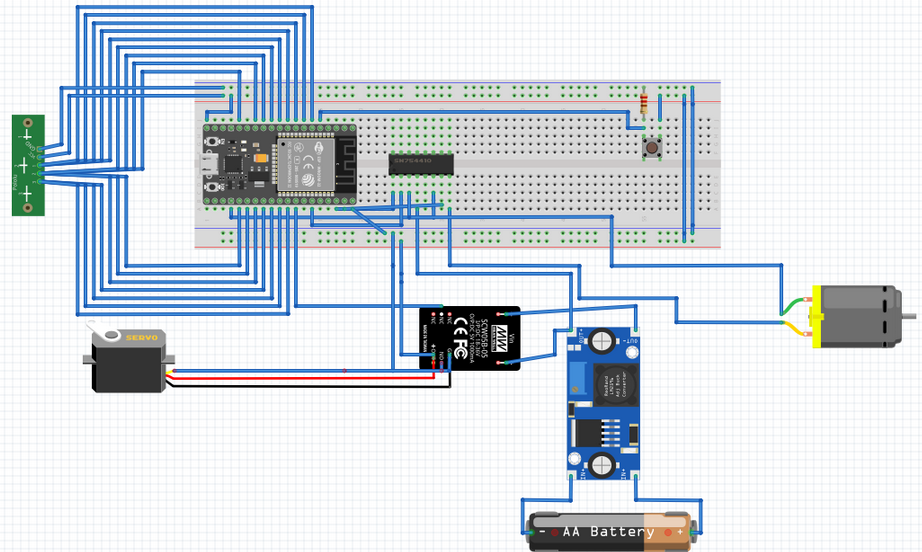
\includegraphics[scale = 0.6]{aufbauSchaltung}
	    	\caption{Aufbau der Schaltung}
	    \end{figure}
	    
        \subsubsection{Aufbau des Servos}
        
            Die Gewindestangen werden mit den beiliegenden Kugelköpfen versehen. Die kürzere der beiden Schubstangen wird später am Servo montiert. Hierfür muss zusätzlich der Servoarm an der kurzen Stange befestigt werden. Die Mittelstellung am Servo sollte ungefähr so positioniert werden. Um die Montage zu erleichtern, wird der Servoarm wieder vom Servo getrennt.
            Die oberen Haltewinkel für die Achsschenkel werden mit den Messingabstandshaltern und der Bodenplatte verschraubt. Anschließend. Der Servo wird mit den beiden Winkeln ebenfalls an der Bodenplatte befestigt.\cite{roboter-bausatz.de2WDRCSMART2020}
			
        \subsubsection{Arretierung des Lenkgestänges}
            Die Achsschenkel werden von oben und unten durch die Bleche mit dem Chassis verschraubt. Sobald die Servo-Mittelstellung ermittelt wurde, kann die Schubstange für die Lenkung befestigt werden. Das Chassis sollte nun so aussehen. Die Motorleitungen können jetzt angelötet werden, der feste Einbauort an der Hinterachse erleichtert die Lötarbeit. Beim Befestigen der Reifen ist darauf zu achten, dass alle Reifen spielfrei und leichtgängig sitzen. Dabei besonders auf den Zahnradantrieb achten, so dass hier etwas Abstand zum Gummi besteht.\cite{roboter-bausatz.de2WDRCSMART2020}\\
            
        	Der nächste Schritt war, den Kabeln am Motor anzulöten, wobei das Ganze im Labor geschah. Der letzte Schritt bei dem Aufbau der Bauteile des Fahrzeuges war die Montageplatten zu befestigen. Die oberen Montageplatten werden wieder mit Messing-Abstandshaltern versehen und auf der Unterseite des Chassis in den vorgesehenen Bohrungen verschraubt.\\
        	
			\begin{figure}[H]
				\centering
				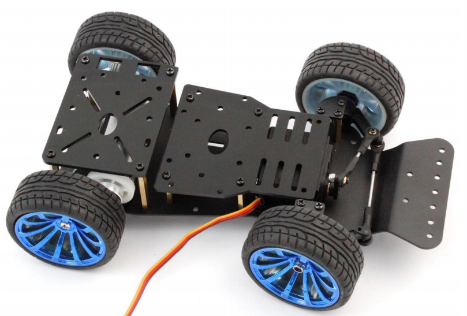
\includegraphics{img/Endergebnis.png}
				\caption{Fertiges Fahrzeug \cite{roboter-bausatz.de2WDRCSMART2020}}
				\label{fahrzeug}
			\end{figure}
        
        
        \subsubsection{Probleme beim Aufbau}
            Das erste Problem hatten wir bei den Schubstangen. Wir haben es übersehen, die Schubstangen so zu verschrauben, dass die vorderen Räder gerade sind. Nachdem wir das Fahrzeug aufgebaut haben, ging es zur ersten Testfahrt. Der Motor hat sich gedreht, jedoch ist das Fahrzeug nicht gefahren, weil wir vergessen haben, die inneren Motorschrauben anzuschrauben. Außerdem war der Abstand zwischen einem der hinteren Räder und Motor zu klein, sodass sich das Rad am Motor geschliffen hat.
            
	\subsection{Antrieb}
		
	\subsubsection{Aufbau}
		
		Der Motor sitzt hinten im Auto zwischen den beiden  Reife und wird von zwei Bords gesteuert:
		
		\begin{itemize}
			\item Das erste Bord ist die H-Brücke, welche die beiden Pins steuert, und dem Motor das richtige Signal weiter gibt, über das die Geschwindigkeit gesteuert wird. 
			\item Der Spannungsregler ist das zweite Bord.Die Aufgabe dieses Bords ist es, dem Motor die richtige Spannung zu liefern.
		\end{itemize} 
	
		
		
		Der Motor braucht 9 Volt um zu fahren, die am ende von der H-Brücke kommen.
		
	\subsubsection{Software}
	
		Der Motor besitzt zwei Inputs um steuern des Motors. Erhält der erste Input Analog eine Zahl zwischen 150 und 255, der zweite 0, so fährt das Fahrzeug vorwärts. Vice versa fährt das Auto Rückwärts. Der Wert, den diese Input erhalten korrespondiert mit der Dreh- und somit der Fahrgeschwindigkeit des Autos. 255 ist die maximale Geschwindigkeit. Zusätzlich müssen die Eingänge EEP und ULT der H-Brücke auf High, oder 1, gesetzt werden. Dafür sind mehrere Methoden in unserem Code vorhanden: \\
		
		initial\_motor initialisiert den Motor und muss zu beginn aufgerufen werden.\\
		
		drive\_forward Steuert die Geschwindigkeit des Motors. \\
		
		int drive\_backward(int value) analog zu drive\_forward, jedoch in die andere Richtung.\\
		
		int turn\_motor\_off stoppt den Motor.\\
		
		Damit das Fahrzeug nicht gleich nach dem anschalten losfährt, muss erst eine Taste auf dem Bredboard gedrückt werden. 
		
	\subsection{Lenkung}
	\label{Lenkung}
	
	\subsubsection{Hardware}
    	Das Fahrzeug wird mithilfe des Servomotors gelenkt, der vorne am Chassis befestigt ist. Der Servo lässt sich in beide Richtungen drehen. Nach dem Aufbau des Fahrzeuges hat man jetzt den Servoarm so befestigt, dass er die vordere Achse mit dem Servo verbindet und somit jede Drehung des Servos die Räder je nachdem nach links oder nach rechts lenkt. \\
    	
        Der Servomotor besitzt drei Kabeln, die am Board angeschlossen werden. (Ein Kabeln für die Stromversorgung und Erdungspin und das dritte für den PWM-Pin). Der Servo ist an Pin 19 angeschlossen.\\
        
        Da der Servomotor 5 V braucht, um den Servo zu drehen, wird zunächst ein Spannungsregler benötigt, der zwischen dem Servomotor und den Batterien angeschlossen wird.
        Die Aufgabe dieses Spannungsreglers ist es, von den ca. 10 V, die von dem Spannungsregler des Antriebsmotors kommen, 5 V für den Servomotor sowie den ESP32 zu schaffen.
        Bevor wir zu der Software kommen, schaffen wir uns einen Blick in die Funktionsweise des Servos.\\
        
    \subsubsection{Funktionsweise des Servos}
    \label{FuktionsweiseServo}
    
        Der Servo ist ein kleines Gerät, das eine Antriebswelle hat. Der Servo wird gesteuert, indem ihm ein codiertes Signal gesendet wird. Dieses Signal in der Eingangsleitung beschreibt dann die Winkelposition. Jedes Mal, wenn sich dieses Signal ändert, dreht sich der Servo um die neue Winkelposition. Der Servo dreht sich normalerweise zwischen 0 – 180 Grad.\\
        
        In der Regel könnte man kleinere Servomotoren direkt am Arduino anschließen, da diser Servo jedoch größer ist, musste er mithilfe des Spannungsreglers an den Batterien angeschlossen werden, um genug Power für den Motor zu haben. Der Servo verfügt über einige Steuerkreise und ein Potentiometer (einen variablen Widerstand), der mit der Ausgangswelle verbunden ist. Dieses Potentiometer ist für die Überwachung des aktuellen Winkels zuständig. Jedes Mal, wenn ein neues Signal kommt, wird überprüft, ob der Servo gerade in der richtigen Position ist. Ist dies der Fall schaltet sich der Motor ab, da eine Drehung nicht nötig ist, anderenfalls dreht sich der Servo in die richtige Winkelposition.\\
        
        Der Steuerdraht wird dafür verwendet, um den Winkel mitzuteilen. Der Winkel wird durch die Dauer eines Impulses bestimmt, der an den Steuerdraht angelegt wird. Dies wird als pulscodierte Modulation bezeichnet.\\
        
        Der Servo erwartet alle 20 ms einen Impuls, es besteht eine Wartezeit von 20 ms zwischen den verschiedenen Signalen, wobei das automatisch verwaltet wird (Man braucht also im Programm keine delays oder Warten-Funktionen). Der Servo dreht sich anhand der Länge dieses Impulses. Er dreht sich z.B. in den Winkel 90 Grad, wenn er einen Impuls mit einer Länge von 1.5 ms bekommt. Bei einem kleineren Impuls als 1.5 ms dreht sich der Servo in Richtung 0 Grad, bei größeren Werten in die andere Richtung also 180 Grad. Und auf dieser Art und Weise dreht sich der Servo zwischen 0 – 180 Grad, was bei dem Fahrzeug dann als Lenkung nach rechts (In Richtung 0 Grad) oder nach links (In Richtung 180 Grad) umgesetzt wird.\\
        
        Man sollte also jetzt den minimalen und maximalen Winkel heraus finden, weil bei höheren Winkeln dreht sich der Servo und, wenn er nicht passend zum Fahrzeug eingestellt ist, bricht der Servoarm.
        Bei unserem Fahrzeug ist dieser Bereich 70 – 140.\\
        
    \subsubsection{Software}
        Man findet in unserem src-Ordner die Datei steeringControl, mit der der Servo gesteuert wird.
        Darin befinden sich zwei Methoden.
        \begin{itemize}
        	
            \item Initializeservo(int pinnum): Nimmt eine Zahl entgegen, welche der Pinnummer entspricht, und aktiviert den Pin mit dieser Nummer, indem der Pin auf OUTPUT gesetzt wird.
            
            \item Turnsurvo(int angle): Diese Methode nimmt eine Zahl entgegen, welche der Winkelposition entspricht. Um das ganze dem Benutzer der Software zu vereinfachen, haben wir hier einen Trick verwendet. Die Zahl angle wird auf die Werte unserer maximalen Grenzen gemappt (70, 140 siehe oben). So kann der Benutzer einen Wert zwischen -35 (voller Lenkeinschlag nach links) und 35 (voller Lenkeinschlag nach rechts) übergeben, welcher dann später in einen Wert zwischen 70 und 140 umgewandelt wird. Gibt der Benutzer z.B. 0 über, so wird der Servo in die Winkelposition 105 gedreht. Bei -35 wäre die Winkelposition 70, und bei 35 wäre die 140.
            Wichtig ist, dass der Wert auf die jeweiligen Grenzen überprüft wird, um Fehler beim Lenken zu vermeiden.
            Der Wert wird dann als codiertes Signal in die Eingangsleitung gesendet (siehe \autoref{FuktionsweiseServo}).
            
        \end{itemize}

    \subsubsection{Probleme beim Servo}
        
            Nachdem wir den Servo angeschlossen haben, ging der Servo zu einem unbekannten Grund defekt. Es hat viel Zeit gekostet, bis wir festgestellt haben, dass es am Servo liegt.
            Wie wir drauf kamen, ist, dass wir mithilfe eines Messgerätes und einem passenden Programm überprüft haben, ob die richtigen Signale bei dem Servo ankommen.
            Lösung: Der Servo musste ausgetauscht werden, und dann ging es wieder.\\
            
            Maximale Lenkung: bei dem ersten Lenkversuch war der Servoarm am Servo befestigt und wir haben in einen höheren Winkel als 140 Grad drehen lassen, das führt dazu, dass der Servoarm von dem Servo gelöst wurde, jedoch endete es nicht so schlimm, weil der Winkel nicht so hoch war.

	\subsection{Sensorik}
	
	\subsubsection{Grundidee hinter dem Sensor}
	
	\begin{figure}[H]
		\centering
		\label{SensorTitel}
		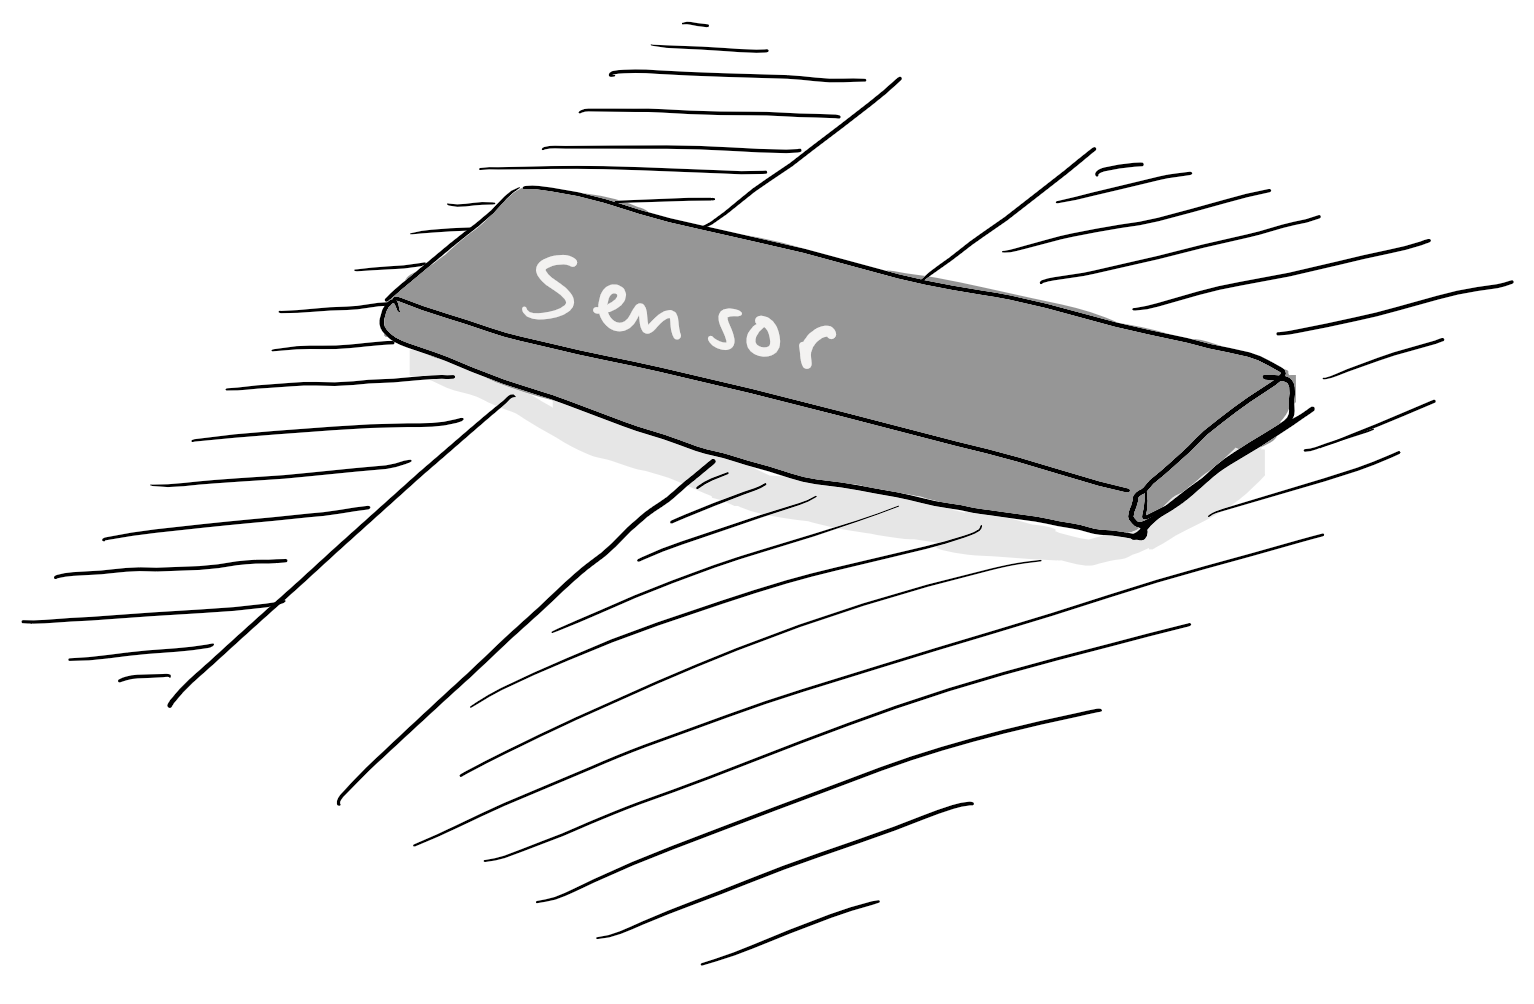
\includegraphics[scale=0.5]{img/Sensor/Sensor1.png}
		\caption{Reflexionssensor auf der Fahrbahn.}
	\end{figure}
	
	
	Die Hauptaufgabe des Sensors ist es, die Linie zu erkennen auf der das Auto am Ende fahren soll. Wir erwarten also, dass wir am Ende den Sensor über die Linie halten, und er auf dem Computerbildschirm eine Repräsentation der Linie in Echtzeit ausgibt. Wie könnte eine solche Repräsentation aussehen? Wir haben uns für eine Folge von Nullen und Einsen entschieden:
	
	\begin{figure}[H]
		\centering
		\label{sensor2}
		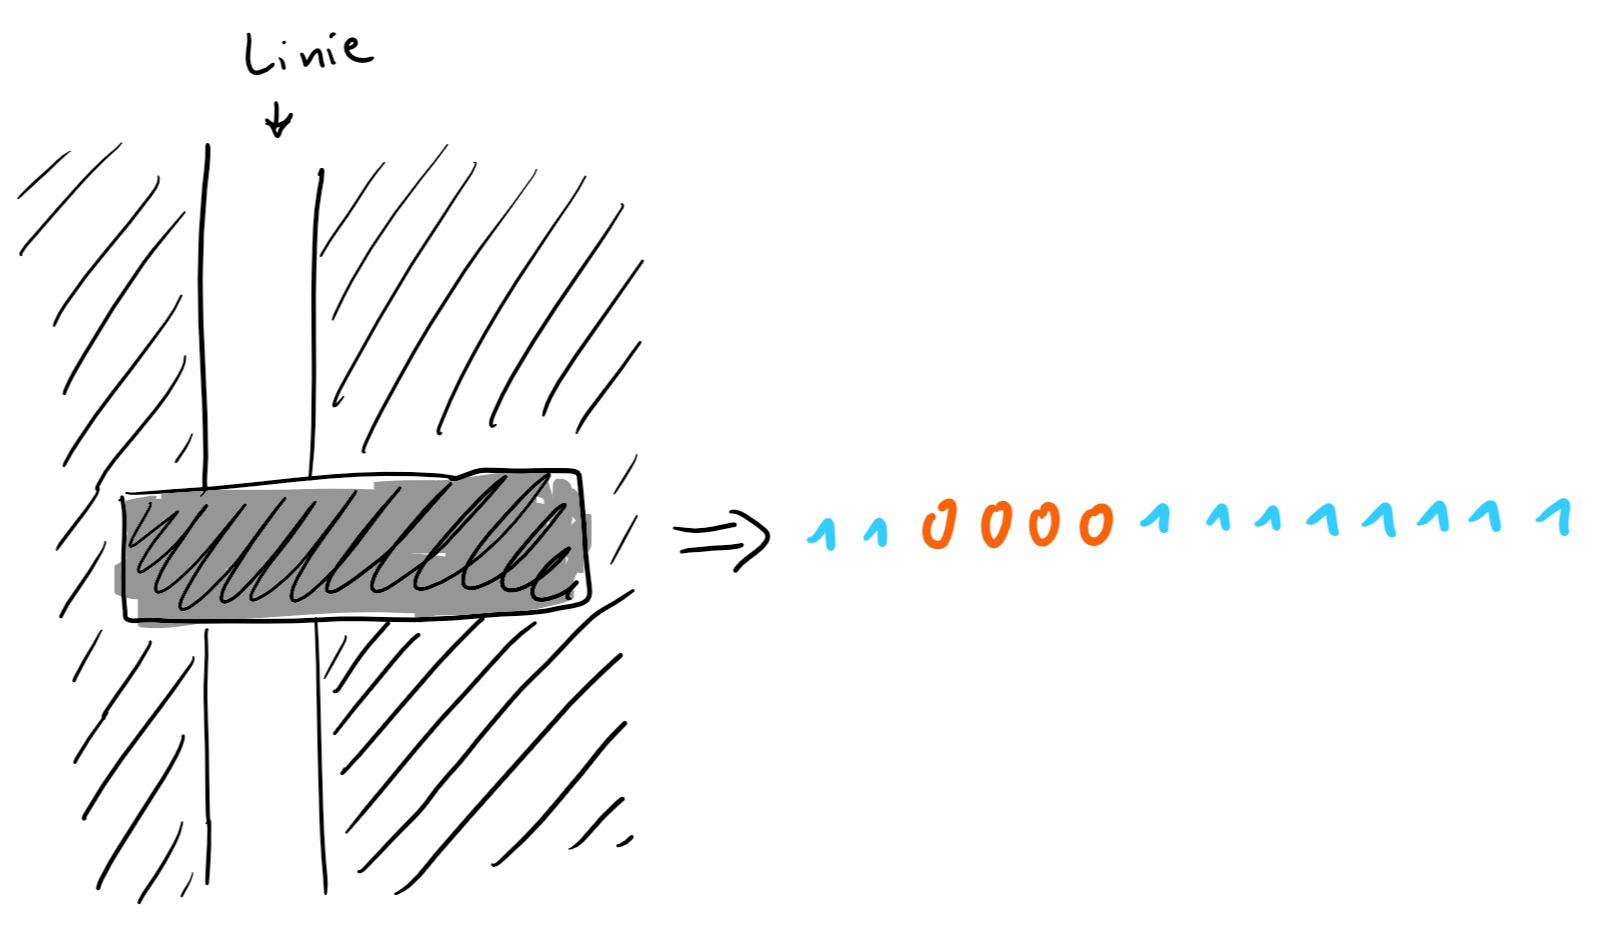
\includegraphics[scale=0.5]{img/Sensor/Sensor2.png}
		\caption{Sensor in Aktion mit entsprechender Ausgabe.}
	\end{figure}

	
	 
	 Als Repräsentation dient also eine Bit-Folge. Dort wo die Nullen sind ist die Linie.
	 Wenn wir den Sensor horizontal über die Linie bewegen, so erwarten wir eine entsprechende Veränderung im Bit-Muster.
	 
	 \begin{figure}[H]
	 	\centering
	 	\label{sensor3}
	 	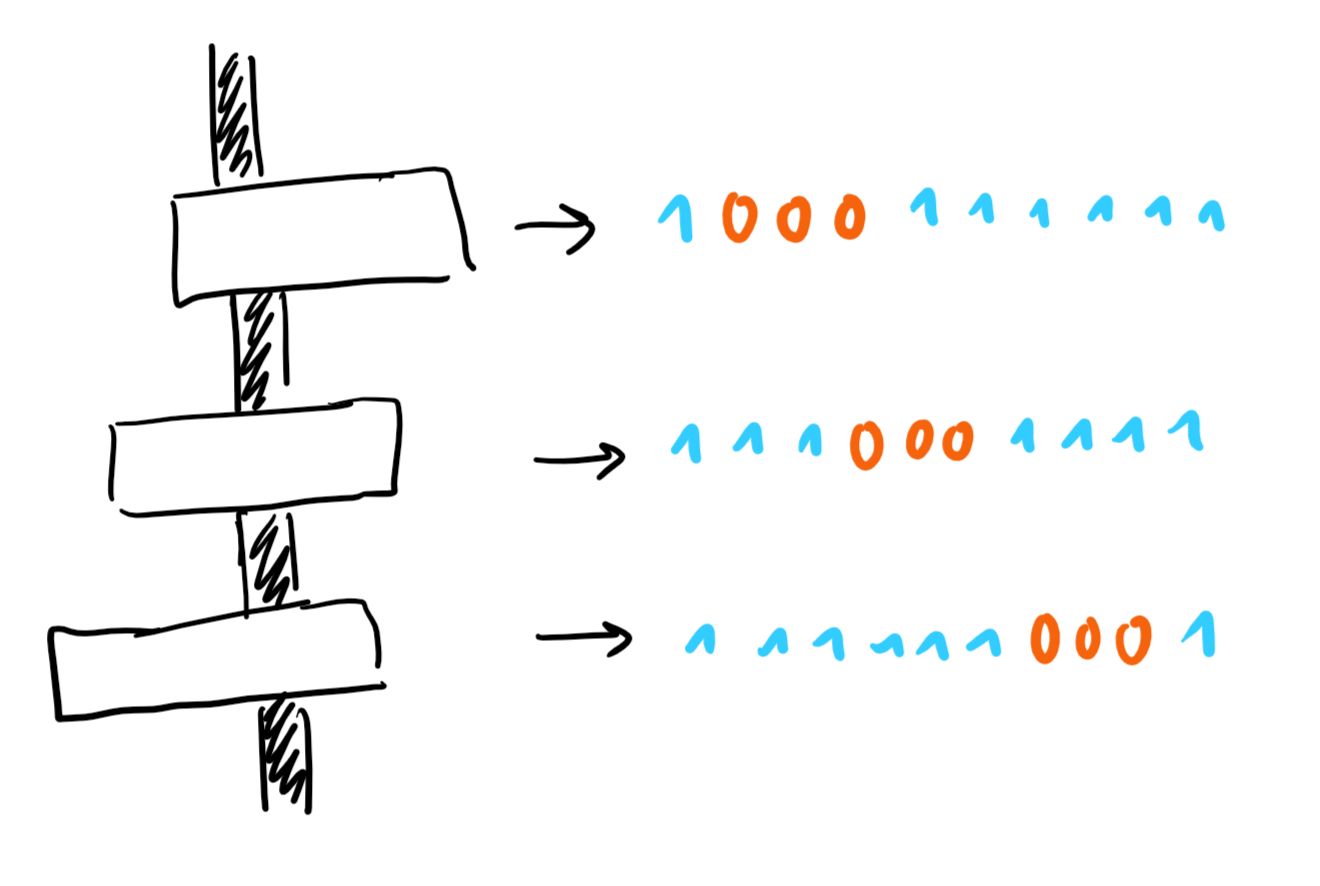
\includegraphics[scale=0.5]{img/Sensor/Sensor3.png}
	 	\caption{Verschiedene Ausgaben je nach Sensorposition.}
	 \end{figure}

	 
	 Hier wären auch andere Codierungen denkbar. Z.B. 0 = schwarz und 1 = weiß. Wir haben uns für diese Variante entschieden, da die Hardware diese Werte liefert. Das wird später klar werden.
	 
	\subsubsection{Sensor Hardware}
	 Für das Projekt wurde als Hardware eine spezielle Sensorleiste vorgegeben, der sogenannte QTRX-HD-15A Reflectance Sensor Array. Hier ist der Link zu der entsprechenden Homepage: \href{https://www.pololu.com/product/4415}{\textcolor{blue}{https://www.pololu.com/product/4415}}. 
	
	\begin{figure}[H]
		\centering
		\label{Sensor}
		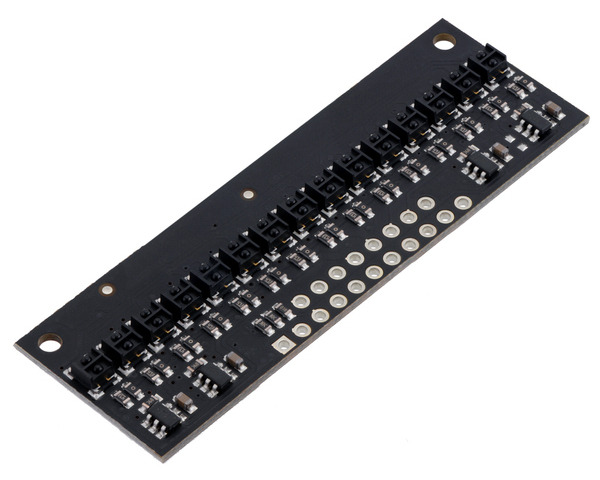
\includegraphics[scale=0.5]{img/Sensor/Sensor.jpg}
		\caption{QTRX-HD-15A Reflectance Sensor Array \cite{poluluQTRXHD15AReflectanceSensor2021}}
	\end{figure}
	
	Wie der Name schon sagt, handelt es sich dabei um eine Aneinanderreihung von Sensoren. Somit war es eigentlich falsch, dass oben von \emph{einem} Sensor geredet wurde, wo doch eine ganze Reihe Sensoren vorliegt.
	\\
	
	Es gibt mehrere Modelle der Sensorleiste. Zu Beginn arbeiteten wir mit einem Modell, wo weniger Sensoren eingebaut waren, um alle benötigten Vorgänge besser zu verstehen. Später nutzen wir dann eine Sensorleiste mit insgesamt 16 Sensoren.\\
	
	Die grundlegende Funktionsweise eines einzelnen Sensors geht wie folgt: Zunächst wird eine LED zum leuchten gebracht. Das Licht trifft auf den Boden und wird reflektiert zu einem Fotowiderstand. Durch diesen soll gemessen werden, wie stark das Licht reflektiert wurde. Und daraus soll abgelesen werden, ob der Sensor einen Schwarzen Untergrund (wenig Licht reflektiert) oder einen weißen Untergrund (viel Licht reflektiert) registriert hat.\\
	
	Die einfachste bzw. naheliegendste Umsetzung dazu sieht wie folgt aus:
	
	\begin{figure}[H]
		\centering
		\label{Sensorfunktion}
		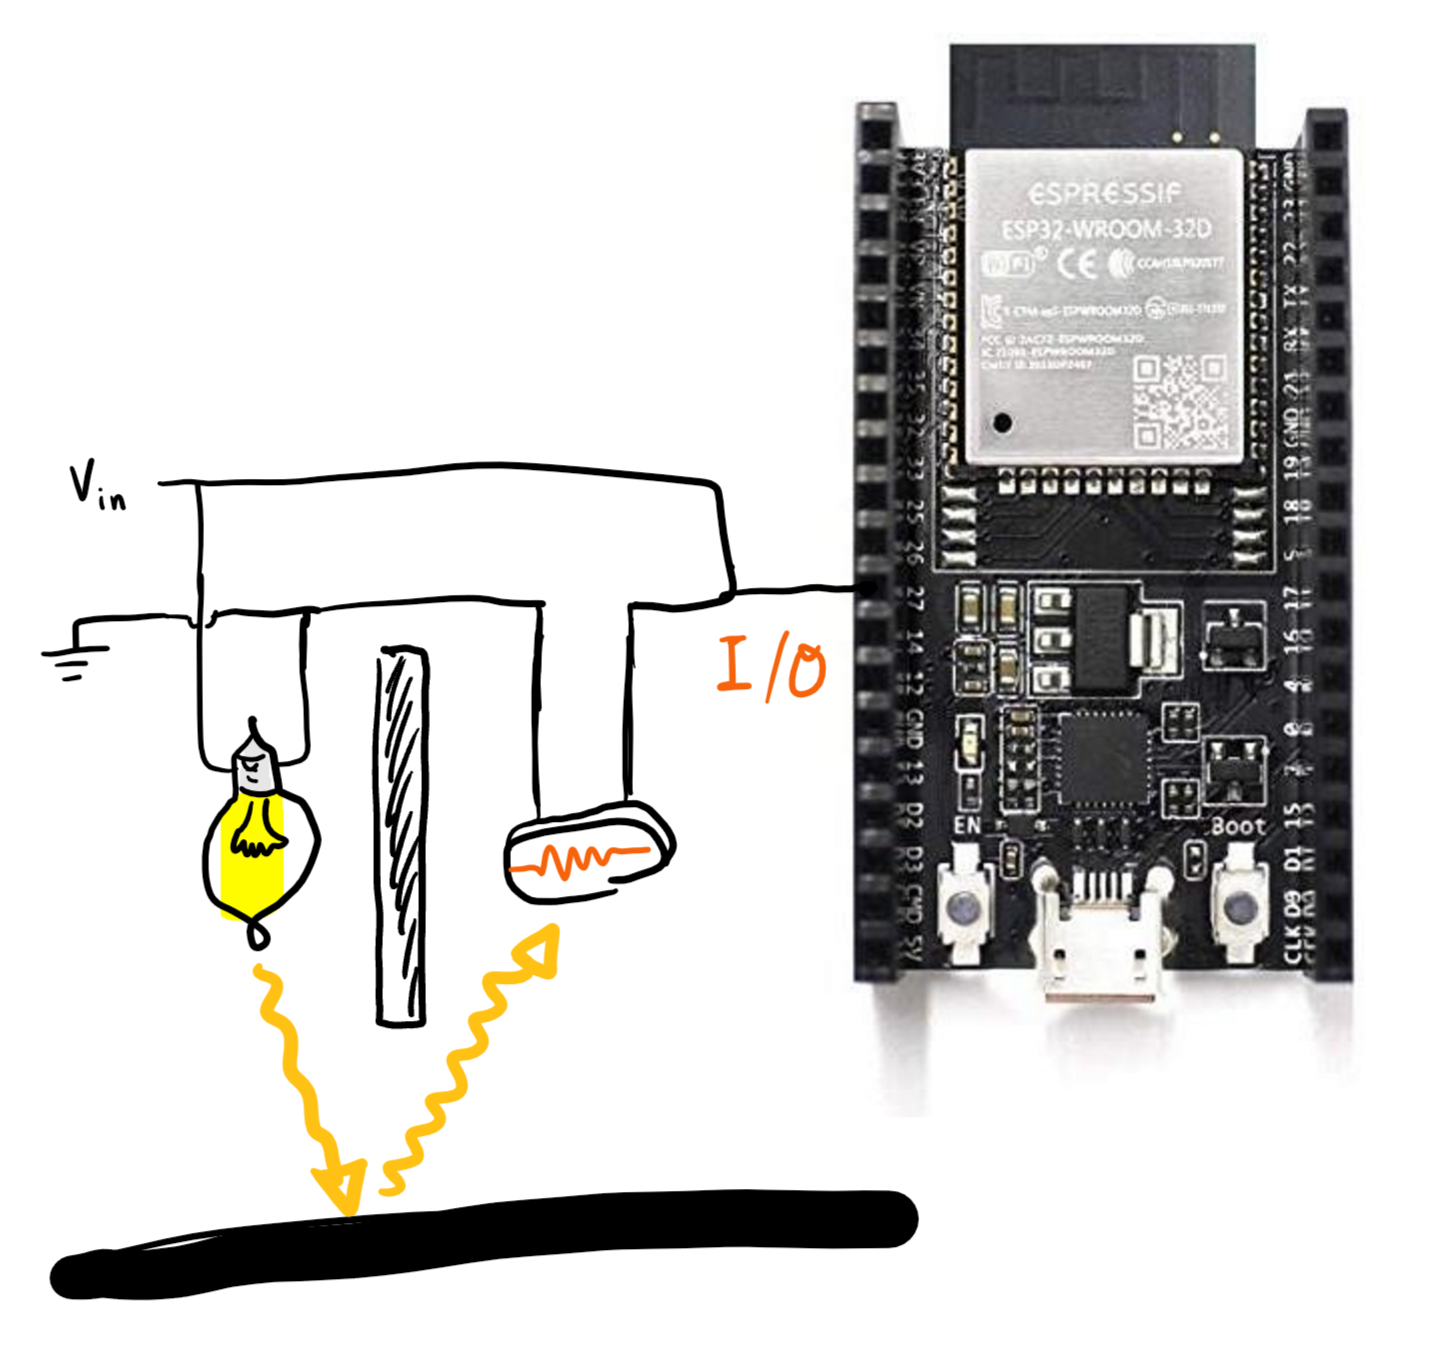
\includegraphics[scale=0.5]{img/Sensor/Sensor4.png}
		\caption{Vereinfachte Darstellung der Funktionsweise des Sensors(ESP32 Abbildung aus 	\cite{ESP32Picture})}
	\end{figure}
	
	Auf der Skizze sieht man die LED mit einer räumlichen Trennung zum Sensor. Die Spannung an der Stelle I/O kann gemessen werden. Wenn viel Licht reflektiert wird (weißer Untergrund), dann hat der Fotoresitor einen geringen Widerstand. An der I/O Stelle kann dann nur eine sehr geringe Spannung gemessen werden (minimal 0V). Andersrum wenn wenig Licht reflektiert wird (schwarzer Untergrund): der Fotoresistor bietet einen hohen Widerstand. Am I/O Pin kann eine hohe Spannung gemessen werden (maximal $V_{in}$).
	
	Wenn man diesen Sensor über eine sich drehende schwarze Scheibe hält die einen weißen Strich aufgedruckt hat, dann sieht die Spannung am I/O Pin etwa so aus:
	
	\begin{figure}[H]
		\centering
		\label{Spannungskurve}
	 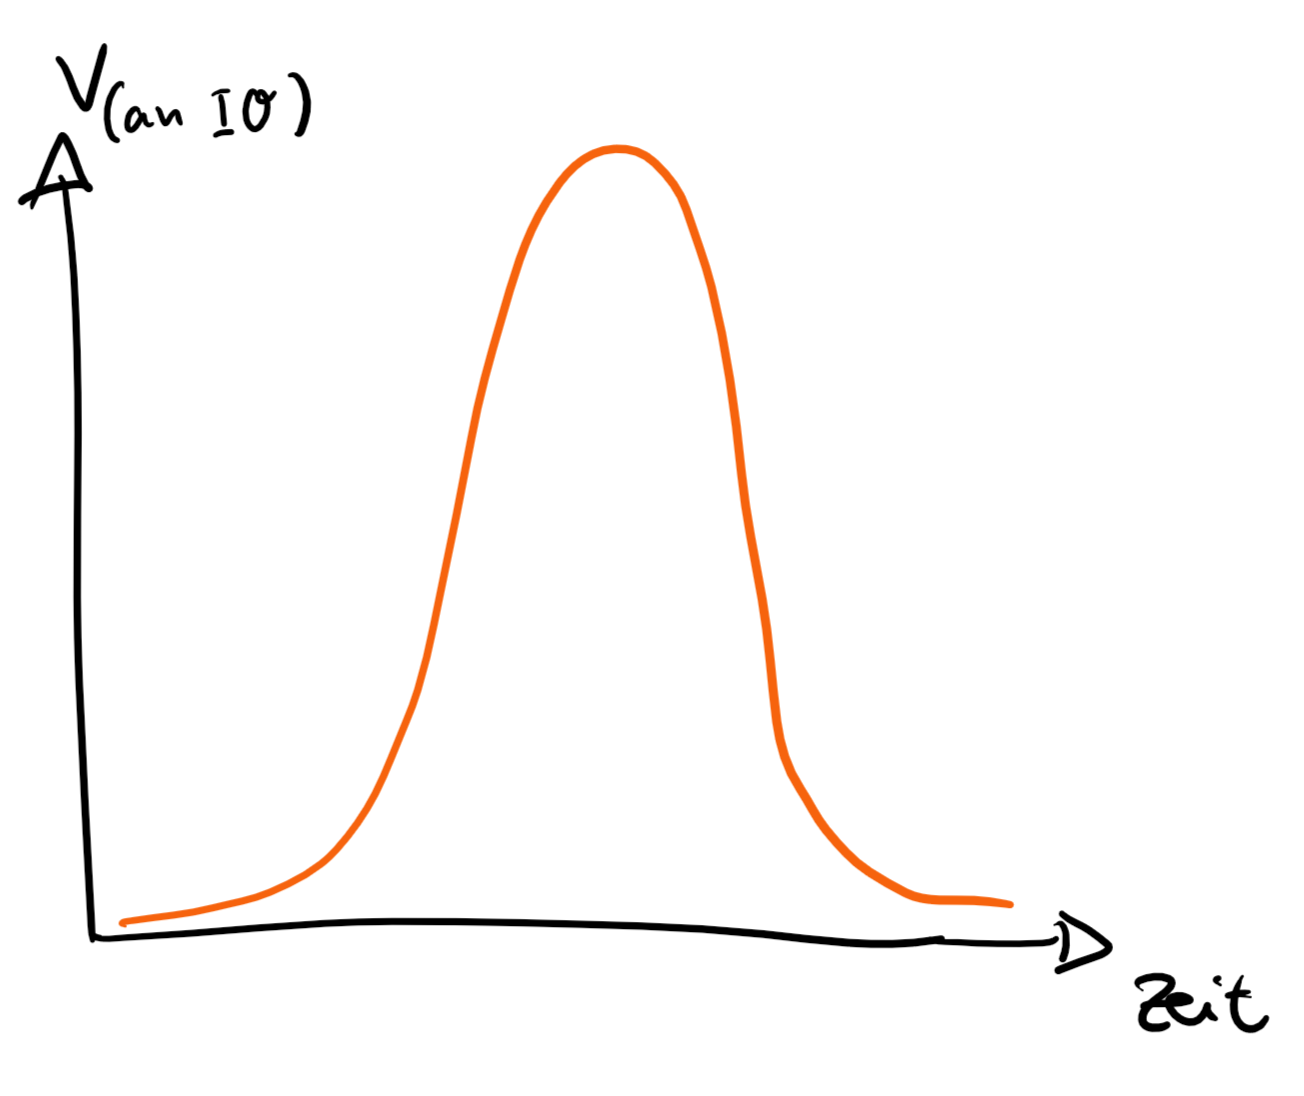
\includegraphics[scale=0.3]{img/Sensor/Sensor5.png}
		\caption{Spannungskurve am Pin}
	\end{figure}
	\newpage
	
	Uns wurde vorgegeben, dass wir mit einem anderen Sensormodell arbeiten sollen. Auch hier gibt es eine LED und einen Fotowiderstand, aber zusätzlich ist ein Kondensator eingebaut, der sich aufladen kann. Die beiden Modelltypen sehen als Schaltplan so aus:
	
	\begin{figure}[H]
		\centering
		\label{schaltplanSensor}
		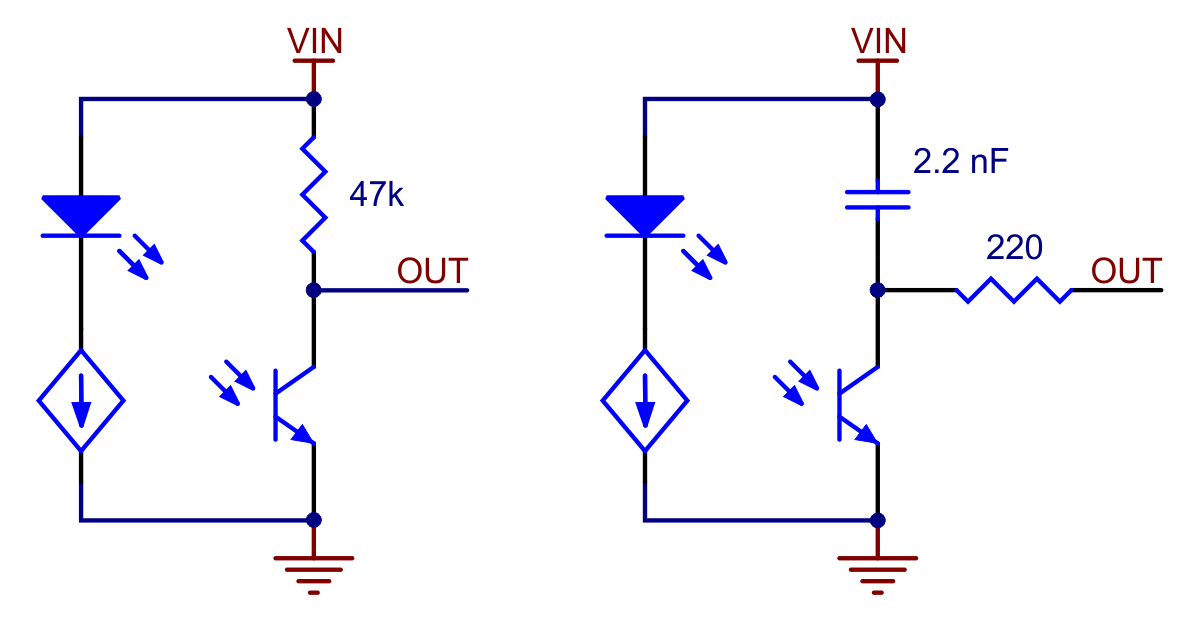
\includegraphics{img/Sensor/Schaltplan.png}
		\caption{Schaltplan der A Version (links) und der RC Version(Rechts) \cite{poluluQTRXHD15AReflectanceSensor2021}}
	\end{figure}
	

	
	Die zuvor als I/O bezeichnete Stelle wird hier OUT genannt. Wir verwenden das hier zum beschreiben synonym.
	Im verbauten RC Modell (hier rechts abgebildet), wird eine Messung wie folgt vorgenommen: Zunächst wird der I/O Pin wie ein Output Pin behandelt und es wird eine Spannung angelegt. Dadurch lädt sich der Kondensator auf. anschließend wird  der I/O Pin zu einem Input-Pin ernannt. Er bietet dabei einen hohen Widerstand. Damit sich der Kondensator entladen kann, muss die Spannung über den Fotowiderstand abfallen. Wenn viel Licht auf den Fotoresistor trifft, dann hat er einen geringen Widerstand und der Abfall verläuft sehr schnell. Wenn wenig Licht drauf triff, dann verläuft der Prozess langsam.
	
	\begin{figure}[H]
		\centering
		\label{entladungKodensator}
		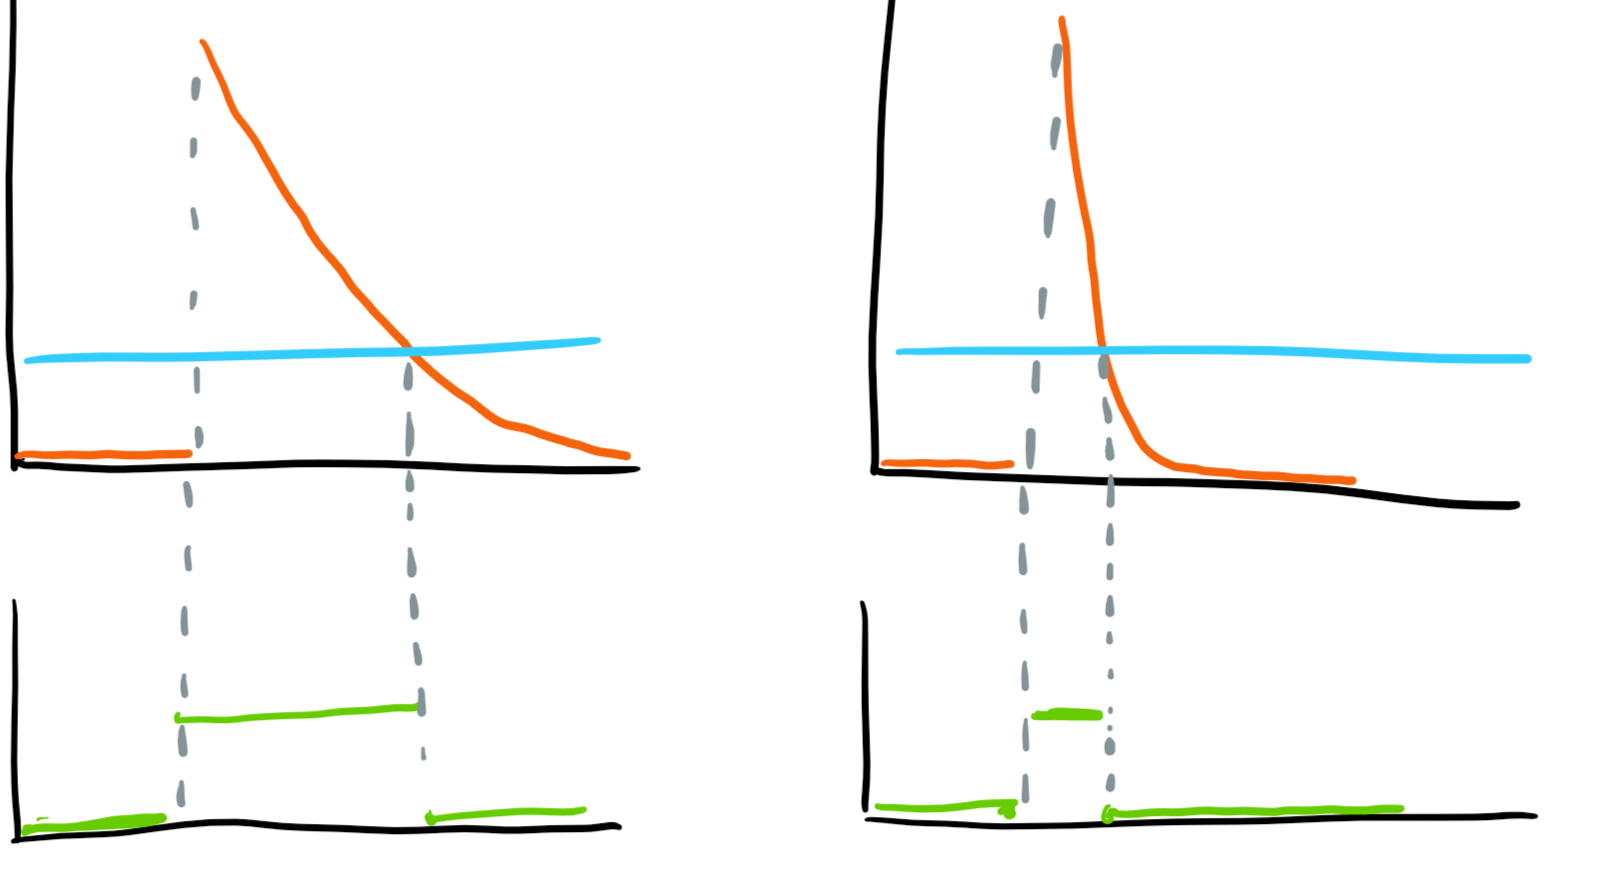
\includegraphics[scale=0.5]{img/Sensor/Kurve2.png}
		\caption{Entladung des Kondensators über die Zeit.}
	\end{figure}

	
	Die Rote Linie zeigt das, was man am I/O Pin messen würde, links für einen schwarzen Untergrund, rechts für einen weißen. Zu Beginn ist die Linie bei 0, da keine Spannung zum I/O Pin gelangt. Wie oben beschrieben wird anschließend der I/O Pin kurz zum Output-Pin und lädt so den Kondensator auf. Das ist in der Abbildung der Fall, sobald die rote Linie schlagartig nach oben geht. Dann wird der I/O Pin zum Input Pin und der Kondensator entlädt sich über den Fotoresistor. Wenn der Widerstand hoch ist (also der Untergrund schwarz), dauert dieser Vorgang länger, als wenn er niedrig (der Untergrund also weiß) ist. Die blaue Linie zeigt, ab wann der I/O Pin tatsächlich eine Eingabe merkt, da er nur zwischen zwei Zuständen unterscheiden kann. Nur wenn die rote Linie über der blauen liegt, kann am I/O Pin eine Eingabe festgestellt werden. Die grüne Linie zeigt dann den tatsächlichen Output, den man beim Messen am I/O Pin bekommt. Die Unterscheidung zwischen schwarz und weiß gelingt nun, indem man nach einer gewissen verzögerung den I/O Pin abfragt, ob eine Spannung anliegt. Diese Abfrage entspricht der grünen Lienie, da der Pin nur zwischen zwei Zuständen unterscheiden kann. Die Frage, wie lange man genau warten muss um ein gutes Ergebnis zu bekommen ist nicht leicht: wartet man zu lange ist der Kondensator in jedem Fall schon entladen und der I/O Pin wird immer 0 zurück geben, egal, was wirklich unter dem Sensor liegt. Schaut man umgedreht zu früh nach, so wird der Sensor immer 1 zurück geben. Wir haben diese zeitliche Verzögerung den "Threshold" genannt. Den richtigen Threshold zu finden soll sich später als kritischer Faktor herausstellen, damit das Auto korrekt lenken kann. 
	  
	  	\begin{figure}[H]
	  	\centering
	  	\label{thresholds}
	  	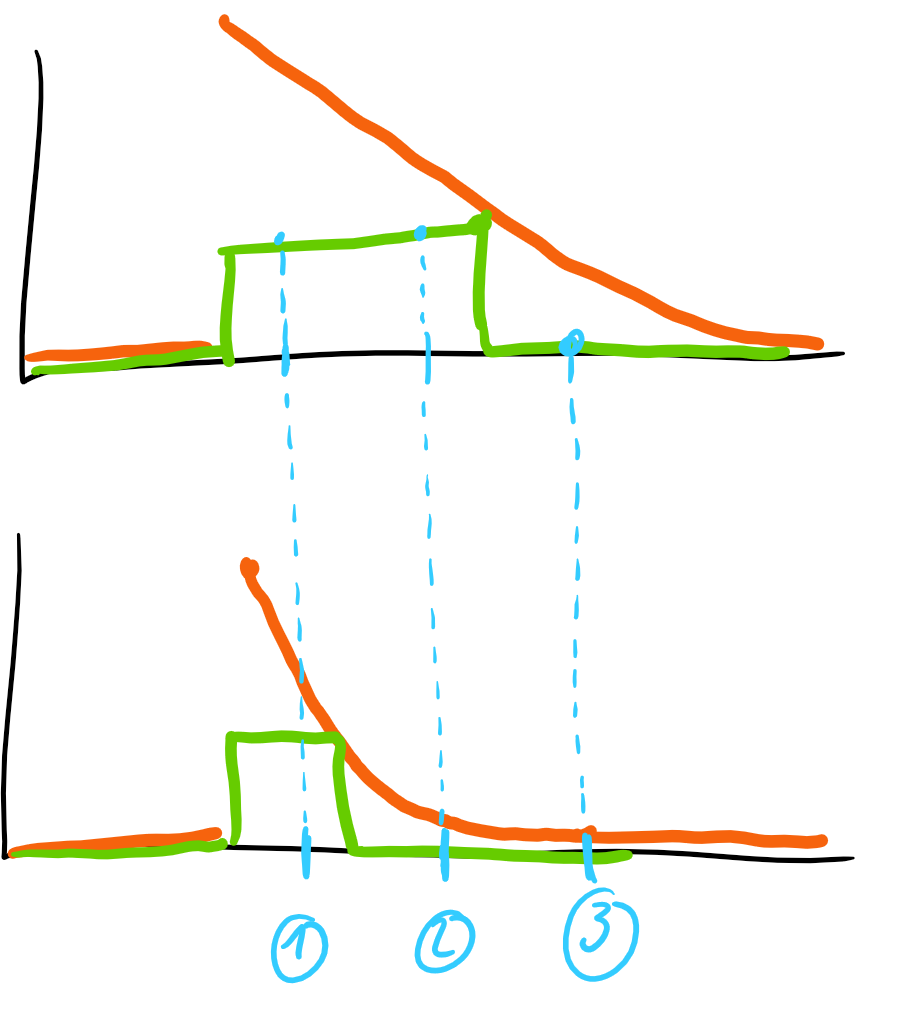
\includegraphics[scale=0.5]{img/Sensor/Kurve3.png}
	  	\caption{Darstellung der Thresholds anhand der Entladungskurve.}
	  \end{figure}

	  
	  Der obere Graph zeigt die Messung bei einem schwarzen Untergrund, die untere bei einem weißen. Die grüne Linie zeigt wieder das an, was der I/O Pin auf Anfrage bei einer Messung zurück gibt. Die Zeitspanne von dem Moment an, wo der Kondensator aufgeladen wird bis zur Messung ist der Threshold. In der Grafik wird an drei Punkten überprüft, ob sie geeignet für einen Thresold wären. Ein Threshold der bis zur (1) geht wäre schlecht, da er immer den Wert 1 liefert. Analoges gilt für (3), hier gibt die Messung immer den Wert 0. Nur bei (2) kann eine sinnvolle Unterscheidung gemacht werden. Es soll sich auch heraus stellen, dass jeder einzelne Sensor auf der Leiste seinen eigenen Threshold hat. Nimmt man eine Änderung an der Hardware vor oder  benutzt das Auto längere Zeit nicht, so muss der Threshold oft angepasst werden. Daher wurde schnell klar, dass es einer vollautomatischen Kalibrierung bedarf, um das Auto angenehm bedienen zu können. Dazu später mehr. Man bemerke nun, dass also ein weißer Untergrund am I/O Pin eine 0 zurück gibt, während ein schwarzer eine 1 zurück gibt. Daher haben wir uns dazu entschieden, an dieser Stelle die Repräsentation auch genau so zu wählen: 0 für weiß, 1 für schwarz.
	  \newpage
	  Auf der Sensorleiste kann man die LED und den Fotoresistor übrigens auch sehen:
	  
	  \begin{figure}[H]
	  	\centering
	  	\label{sensor6}
	  	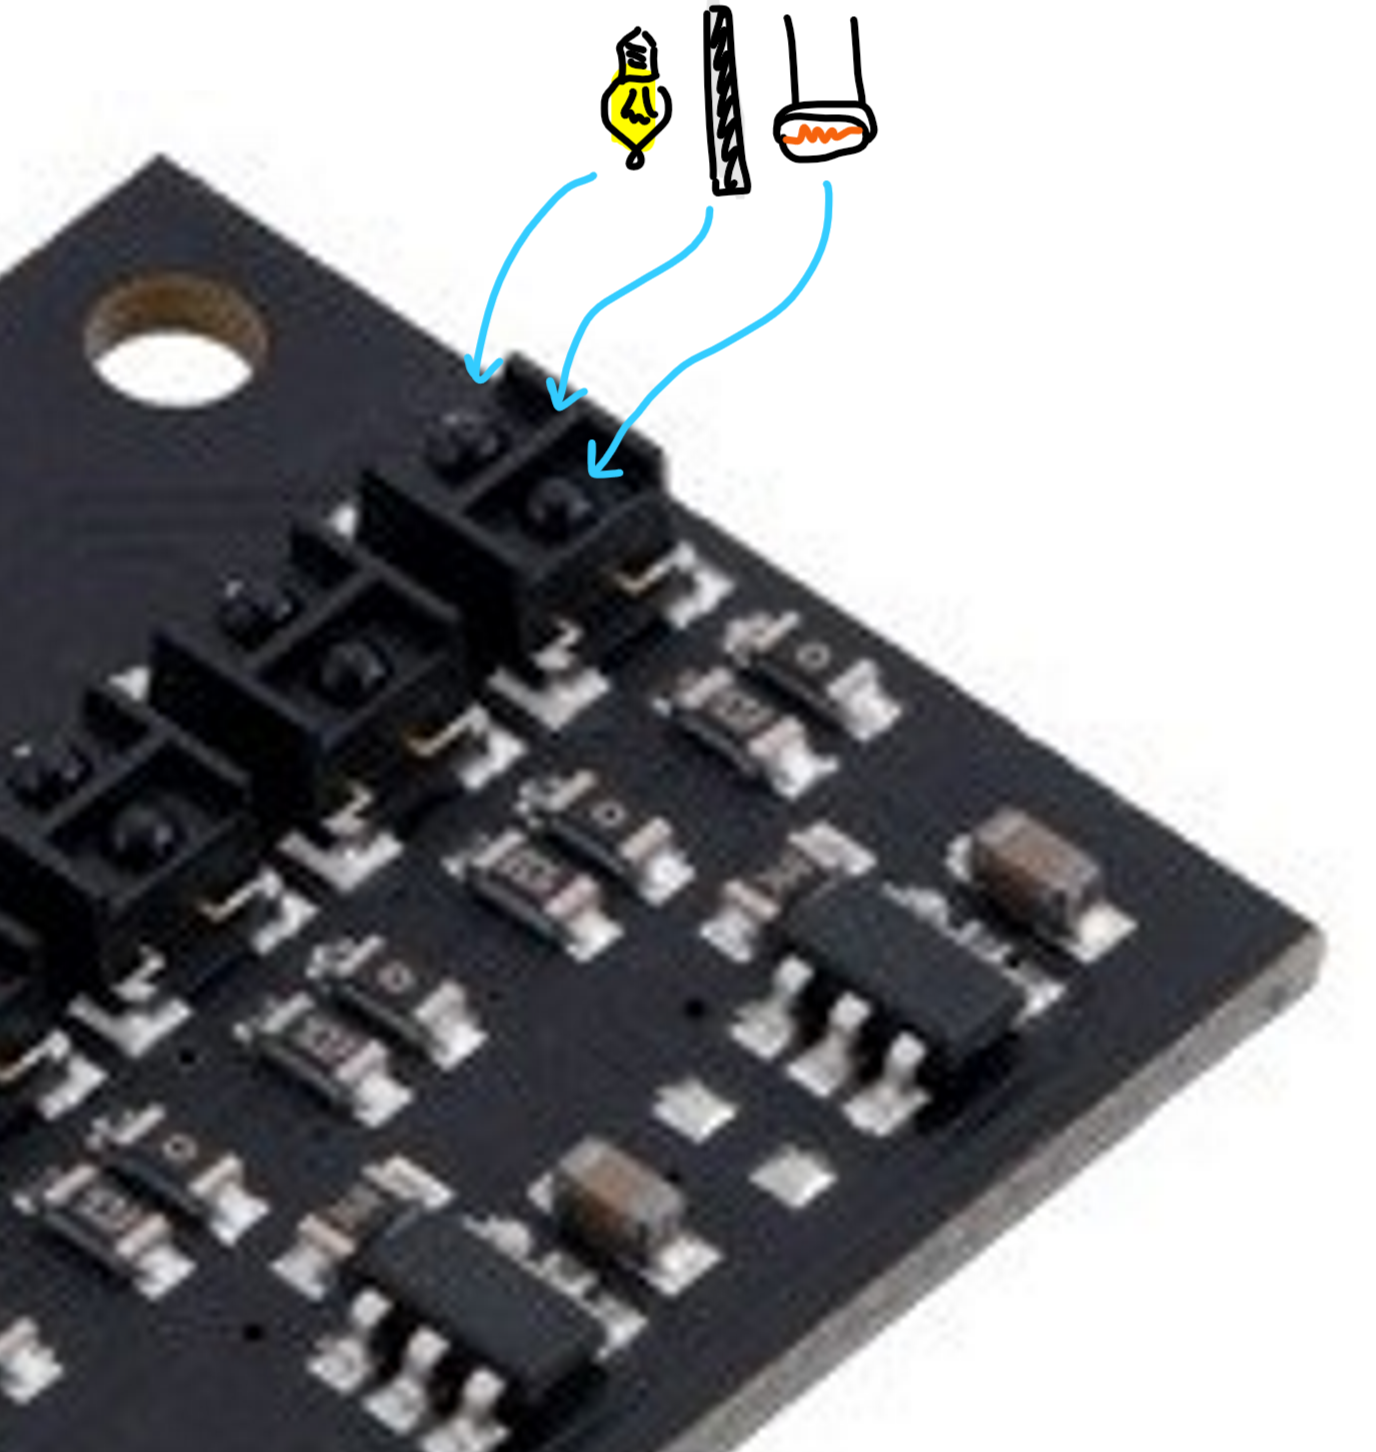
\includegraphics[scale=0.5]{img/Sensor/Sensor6.png}
	  	\caption{Die LED links, der Fotowiderstand rechts und die Trennwand in der Mitte..}
	  \end{figure}
	  
	\subsubsection{Sensorleiste Programmierung}
	
	In einer Schleife werden alle Sensoren nacheinander abgefragt. Die Werte werden dann wie Anfangs angedacht als Bitfolge gespeichert. Da es 16 Sensoren auf der Leiste gibt, wurde hierfür ein spezieller Datentyp uint16\_t genutzt, also eine Ganzzahl mit 16 Bits.
	\\
	
	\begin{figure}[H]
		\centering
		\label{sensor7}
		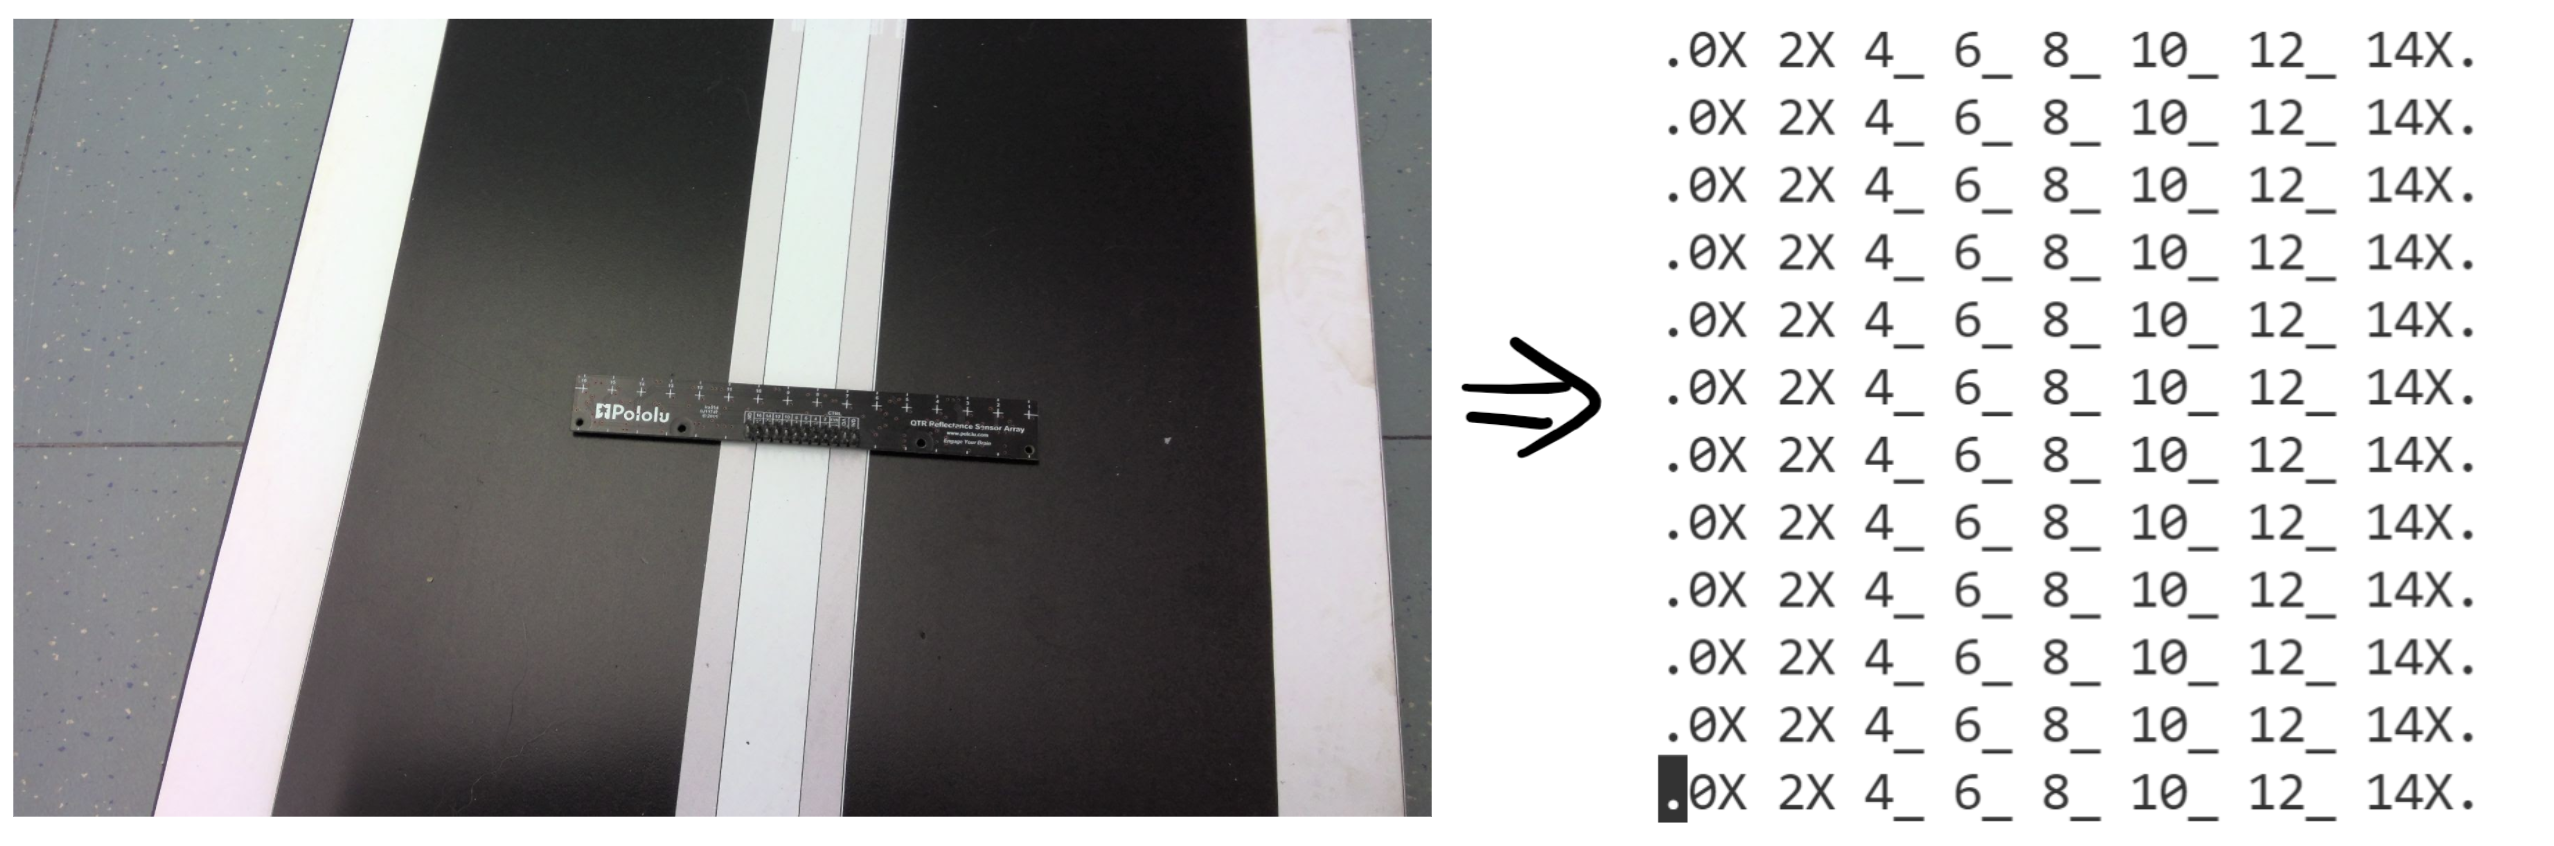
\includegraphics[scale=0.5]{img/Sensor/Sensor7.png}
		\caption{Sensor auf der Fahrbahn mit entsprechender Debug-Ausgabe}
	\end{figure}

	
	Links sieht man den Sensor auf der Fahrbahn. Rechts sieht man das, was zur Überprüfung auf das Terminal ausgegeben wurde:
	Der Sensor wurde hier mehrmals pro Sekunde abgefragt und das Ergebnis wurde in die Konsole ausgegeben. Da der Sensor in dieser Zeit immer das gleiche sieht, wird in jeder Zeile im Terminal das gleiche ausgegeben. Betrachten wir nun eine einzelne Messung, also eine der Zeilen rechts. Was bedeuten die ausgegebenen Dinge? An der Stelle war ich noch nicht soweit, die Ausgabe als eine Zahl aus Einsen und Nullen zu machen. Stattdessen wurde ein ``X" ausgegeben wenn der Sensor schwarz registriert und ein `` \_ ", bei weiß. Die Zahlen davor geben Aufschluss darüber, zu welchem Pin der Output gehört. Steht da z.B. ``0X", dann bedeutet das, dass Pin 1 einen schwarzen Untergrund sieht. Man kann hier auch sehen, dass wir zu Beginn nur jeden zweiten Pin verkabelt haben (denn 16 Stück zu verkabeln ist keine schöne Arbeit). Man bemerke, dass das Foto vom Sensor nur zur Veranschaulichung dient. Eigentlich muss man ihn natürlich verkabeln und ihn festhalten, damit er ein bisschen Abstand zum Boden hat. Dann würde man aber auf dem Foto nicht mehr das wesentliche erkennen.
	\\

	Möchte man die Thresholds neu kalibrieren, sollte wie folgt vorgegangen werden: 
	
	
\begin{enumerate}
	\item  Kippschalter neben dem Batteriefach ausstellen. Sonst liegt gleich die ganze Spannung am USB Port vom Laptop.
	\item  ESP32 mit Laptop per Kabel verbinden
	\item  Das Programm ausführen (z.B.  über VS Code)
	\item  Wenn man bereit ist zum Kalibrieren einfach Enter drücken
	\item  Anweisungen in der Konsole folgen, also:
	\item Auf schwarzen Grund halten und Enter drücken
	\item Warten bis Meldung in Terminal erscheint
	\item Auf weißen Untergrund halten und Enter drücken
	\item Warten bis Meldung in Terminal erscheint
	\item Nun einfach die USB-Verbindung trennen. Die Werte wurden jetzt permanent auf dem ESP32 gespeichert und werden bis zur nächsten Kalibrierung genutzt. Die Werte bleiben gespeichert, auch wenn man das Gerät ausschaltet.
	
\end{enumerate}
	
	Anfänglich hatten wir die Threshold noch einfach in den Code geschrieben, um erste Ergebnisse zu erzielen. Das erste mal, dass das Einlesen der Sensordaten geklappt hat. 
	
	\begin{figure}[H]
		\centering
		\label{Code1}
		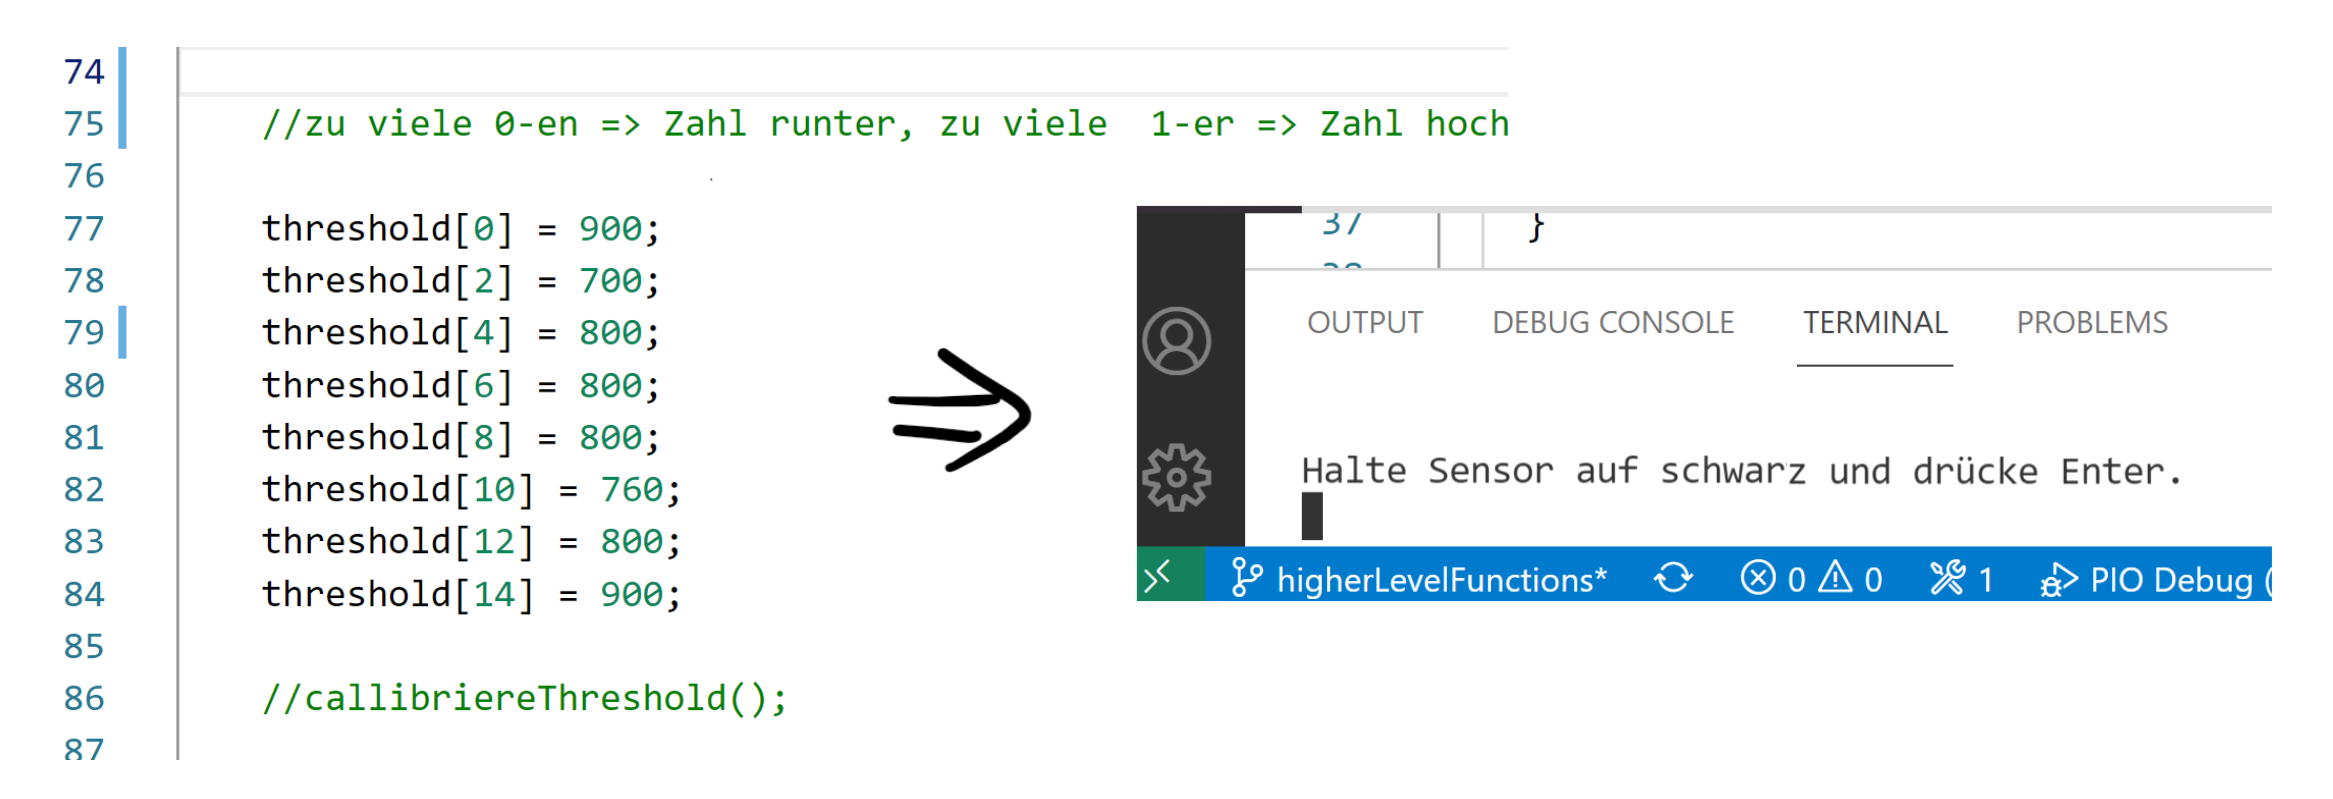
\includegraphics[scale=0.5]{img/Sensor/Code1.png}
		\caption{Kalibrieren der Thresholds über das Terminal}
	\end{figure}

	
	Hier sieht man die Entwicklung: Links noch die Thresholds (in Mikrosekunden) selber durch ausprobieren für jeden einzelnen Sensor in den Code geschrieben. Am Ende vom Projekt wurde die sehr viel bequemere Möglichkeit programmiert, automatisch zu kalibrieren.
	
	\subsubsection{Interpretation der Sensorleiste: Mitte der Linie finden}
	Der erste Schritt des Interpretierens ist nun getan: Aus dem Sensor erhalten wir eine Folge aus Nullen und Einsen. Nennen wir diese mal $x$. Aus denen muss nun aber noch ausgelesen werden, wo die Mitte der Linie ist. Für uns ist das vom drauf schauen sofort klar, dem Computer natürlich nicht. Wie repräsentieren wir am besten die Mitte der Linie? durch eine Zahl zwischen 1 und 16. So bedeutet hier die Zahl 8, dass die Linie genau in der Mitte ist. Nämlich bei Pin 8. Die Zahl 16 heißt, dass die Linie ganz rechts am Rand ist bei Pin 16 und so weiter.\\

	Die einfachste Herangehensweise hierfür ist, $x$ zu durchlaufen und sich zu merken, wo die erste null kommt. Dann wissen wir: Hier fängt der Streifen an. Dann durchlaufen wir die Zahl weiter bis eine 1 kommt und merken uns auch diese Stelle. Hier Endet die Linie. Die Mitte davon ist die Mitte der Linie. Da insgesamt 16 Pins vorliegen, kann diese Zahl auch direkt als Ergebnis ausgegeben werden.
	
	$$x=111 0 0000 1 1111111 = 111\mbox{ } \textcolor{red}{0} \mbox{ }0000\mbox{ } \textcolor{blue}{1}\mbox{ } 1111111$$
	Die rote $0$ ist die erste 0, die blaue $1$ ist die erste darauf folgende 1. Die Positionen lauten 
	$$\Rightarrow 1_1 1_2 1_3  \mbox{ } \textcolor{red}{0_4} \mbox{ } 0_5 0_6 0_7 0_8 \mbox{ } \textcolor{blue}{1_{9}}\mbox{ } 1_{10} 1_{11}  1_{12} 1_{13} 1_{14} 1_{15} 1_{16}\Rightarrow \text{Mitte } = \frac{4 + (9-1)}{2}=6 $$
	$$\Rightarrow \text{Der mittlere Pin ist Pin Numer 6}$$
	In echt funktioniert das aber nicht gut. Man stelle sich vor, einer der Pins hat eine Störung und gibt einen falschen Wert zurück. Hier wurde fehlerhaft eine 0 eingetragen:
	 $$x=1011111110000111$$
	Nun würde der eben beschriebene Algorithmus die erste null als Mitte erkennen und abbrechen. Ich habe daher den Algorithmus angepasst, dass er zu jeder Stelle speichert, wie viele Nullen direkt im Anschluss ohne Unterbrechung folgen. Das würde hier die folgenden Werte ergeben:
	$$1_10_01_01_01_01_01_0\mbox{ } \textcolor{red}{1_4} \mbox{ }0_30_20_10_01_01_01$$
	Die Stelle mit dem höchsten Wert wird genommen und davon ausgehend die Mitte bestimmt. Eine weitere Methode um die Ausrichtung genauer zu machen wäre ein sogenannter PID-Regler. Dieser wurde aber aus Zeitgründen nicht einprogrammiert.
	\subsubsection{Mitte der Linie interpretieren für die Lenkung}
	Nun haben wir eine Zahl zwischen 1 und 16, die uns die Mitte der Linie angibt. Nennen wir diese Zahl $m$.
	\\
	
	Der nächste wichtige Schritt ist, aus der Information, wo die Linien-Mitte ist eine sinnvolle Anweisung für die Lenkung zu machen. Genauer; für den Servomotor. Genaueres dazu im entsprechenden Abschnitt. Aber in Kurzfassung kann man sagen, der Servomotor kann als Input einen Winkel zwischen -35° und +35° entgegen nehmen. 0° bedeutet hierbei, die Lenkung soll geradeaus fahren, 35° scharf rechts und -35° scharf links. 
	\\
	Wenn wir nun wissen, dass die Linie gerade ganz links ist - was müssen wir dann tun? Wie muss gelenkt werden?
	
	\begin{figure}[H]
		\centering
		\label{auto1}
		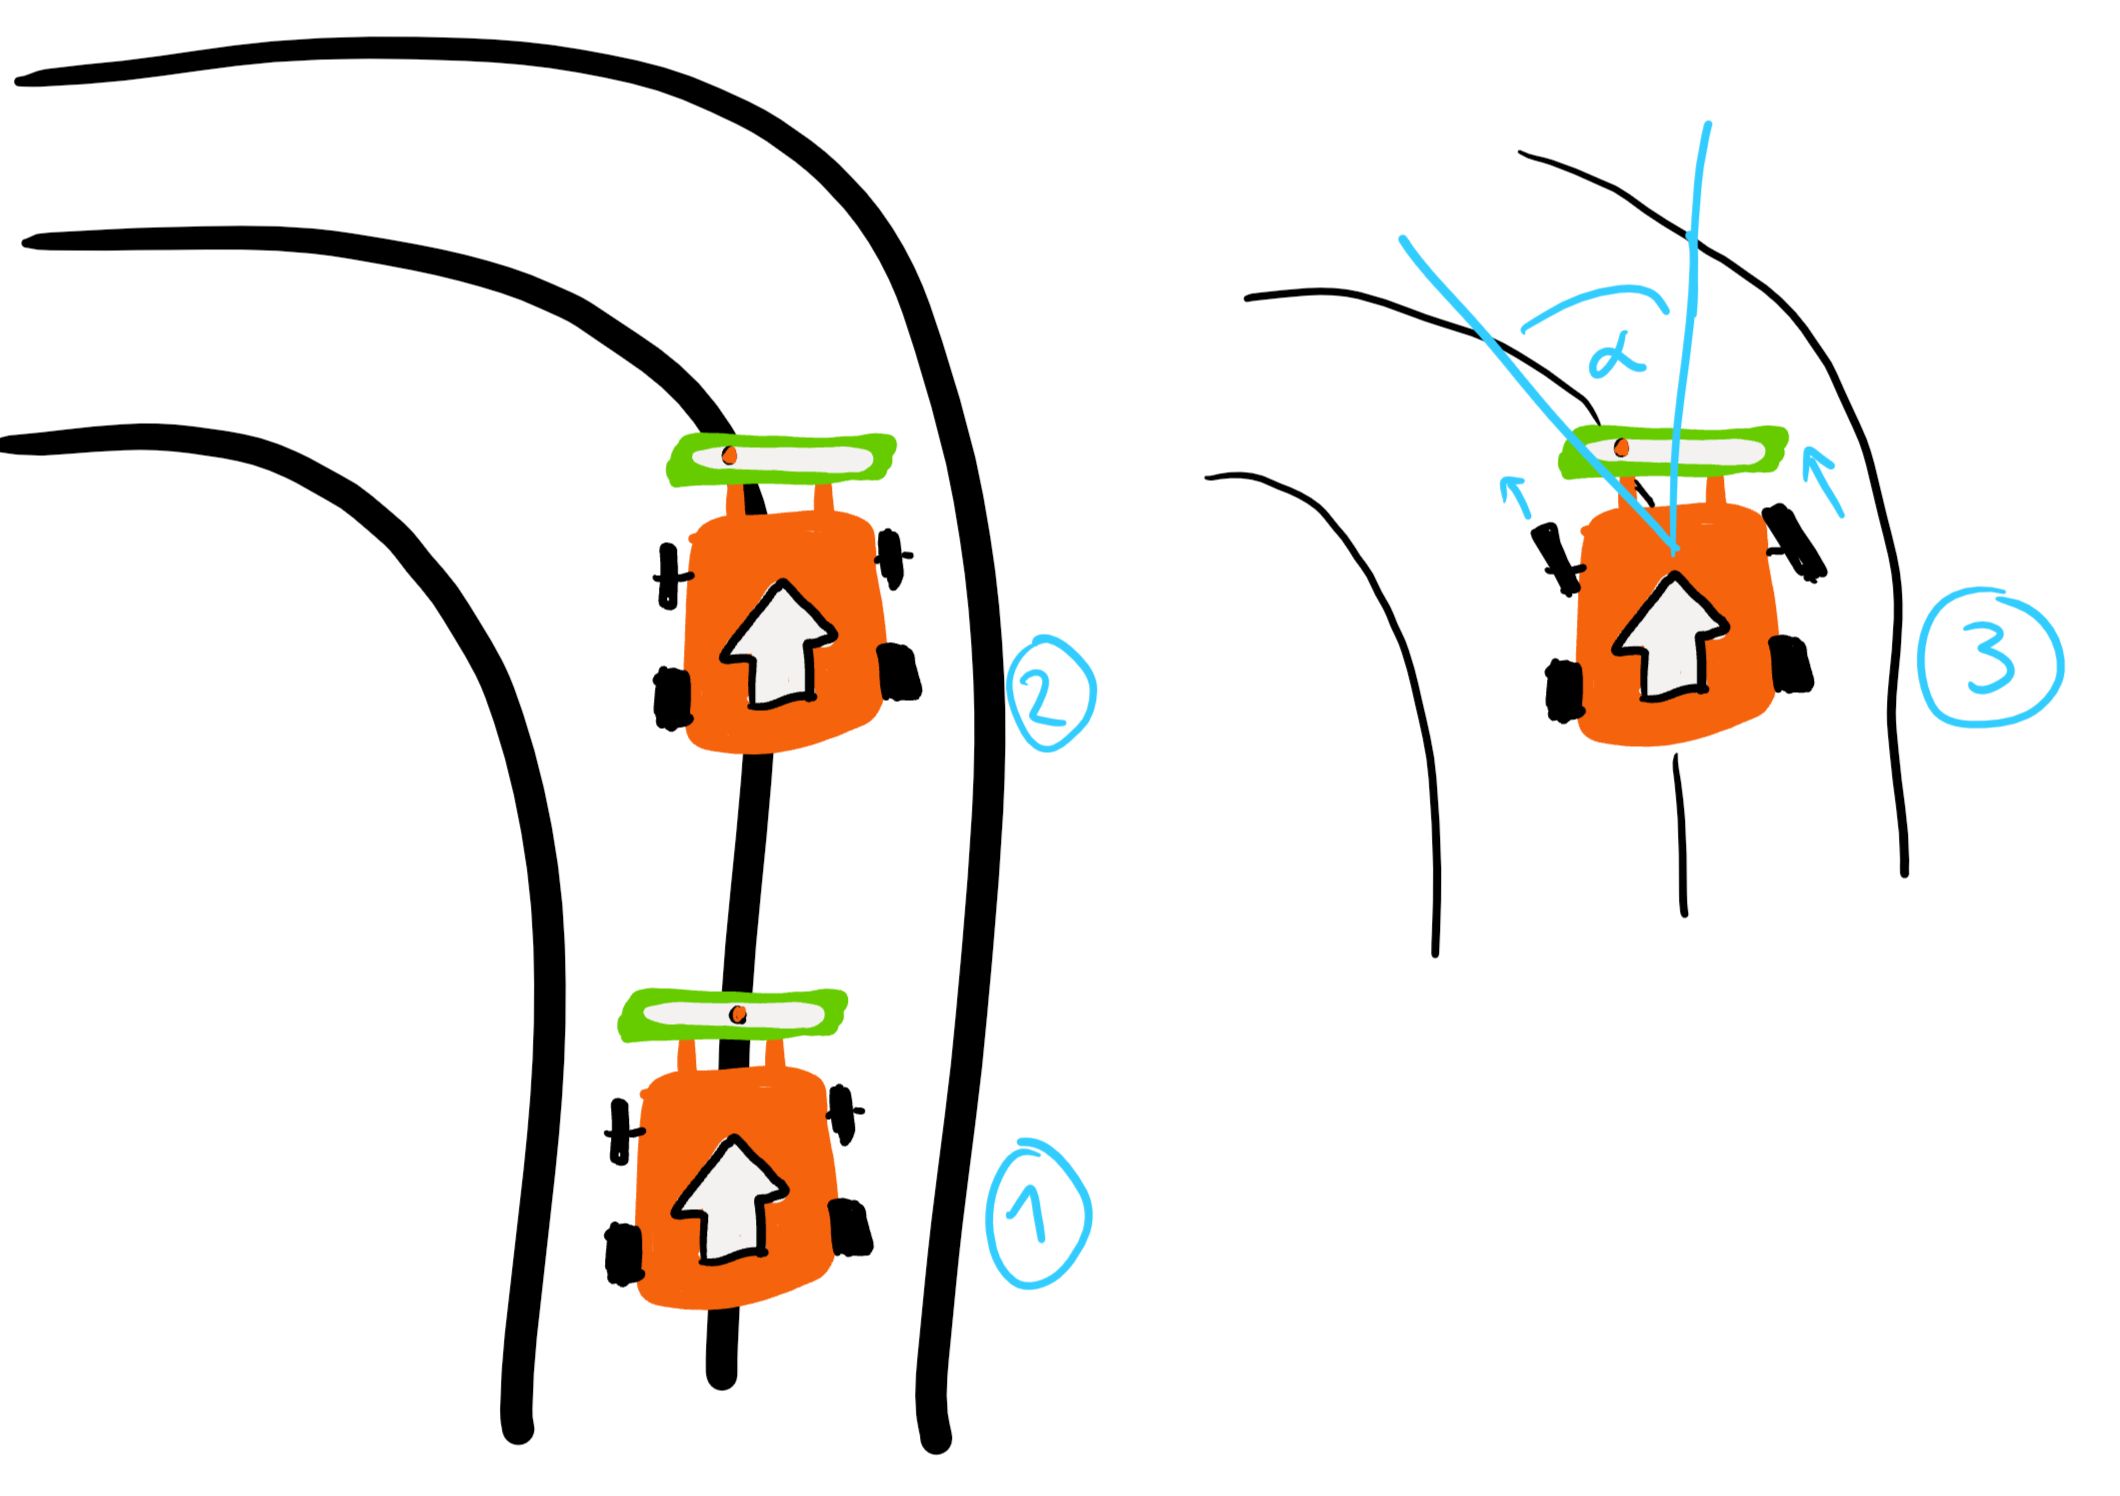
\includegraphics[scale=0.6]{img/Sensor/Auto1.png}
		\caption{Darstellung der aus der Strecke abgeleiteten Lenkung.}
	\end{figure}

	
	Hier sieht man das Auto von oben, wie es über die Strecke fährt, auf eine Kurve zu. An Punkt (1) ist alles o.k. Wenn die Linie bei Pin 8 von insgesamt 16 liegt, also genau in der Mitte, dann muss weder nach rechts, noch nach links gelenkt werden. Es soll also 0° gelenkt werden. An Punkt (2) merkt der Sensor, dass die Linie ganz links außen ist. Wie soll nun gelenkt werden? Die Zeichnung bei (3) zeigt: es muss nach links gelenkt werden, damit das Auto auch nach links in die Kurve fahren kann. Der eingezeichnete Winkel $\alpha$ ist der, den wir suchen. Hier wären 35° sinnvoll. Wohl aber 35° nach links, also muss -35° gelenkt werden. Nach rechts geht das analog.  Wie bekommen wir nun den entsprechenden Winkel? Die naheliegendste Vorgehensweise ist, die Zahlen zwischen 1 und 16 auf die Zahlen zwischen -35 und +35 abzubilden und so den Lenkwinkel zu erhalten. Dafür gibt es eine Funktion namens map:
	$$\alpha = \text{map}(m, 1, 16, -35, 35)$$
	\newpage
	Dabei ist $\alpha \in [-35, 35]$ der Winkel der eingelenkt werden soll. Und $m \in \{1,...,16\}$ die Mitte der Linie. Man kann die Rechnungen, die wir bis jetzt gemacht haben wie folgt zusammen fassen:
	
	\begin{figure}[H]
		\centering
		\label{sensor8}
		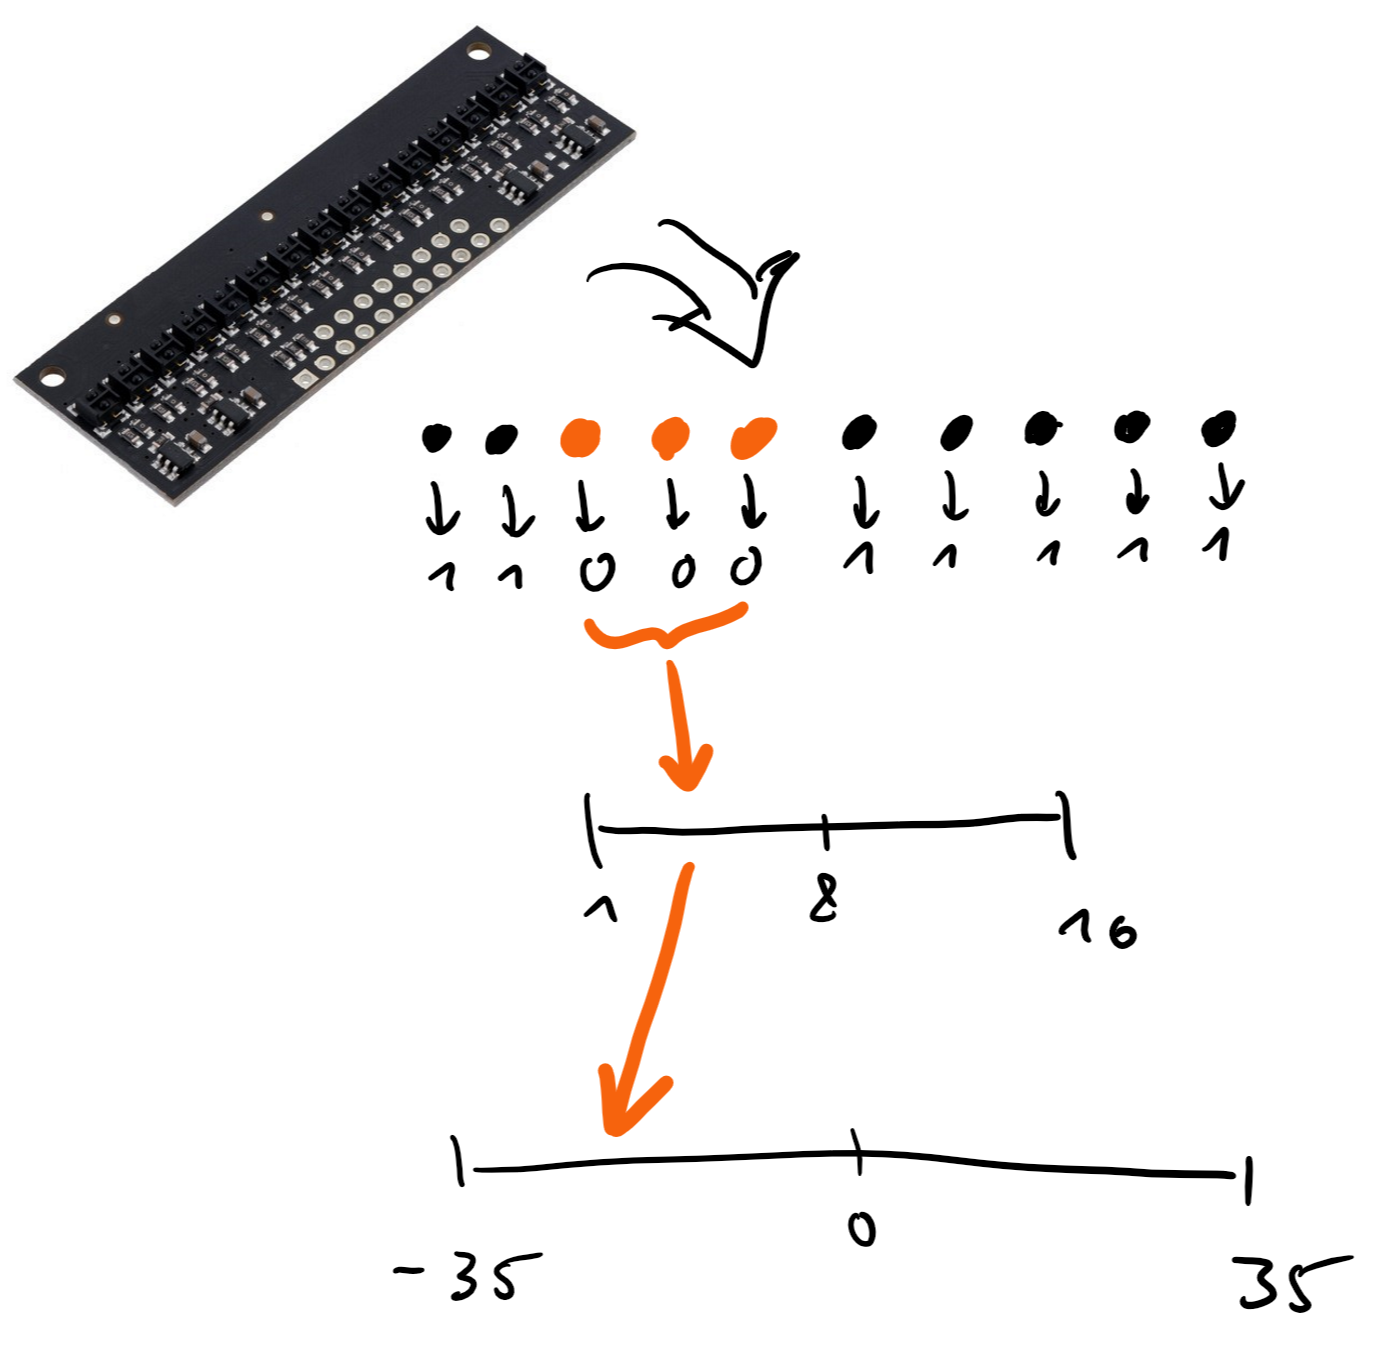
\includegraphics[scale=0.5]{img/Sensor/Sensor8.png}
		\caption{Ableitung des Lenkwinkels aus den Sensordaten.}
	\end{figure}
	
	Ein Problem gibt es bei diesem Ansatz aber noch. Und zwar, was passiert, wenn das Auto in eine Kurve fährt und der Sensor an den Rand kommt?
	
	\begin{figure}[H]
		\centering
		\label{auto2}
		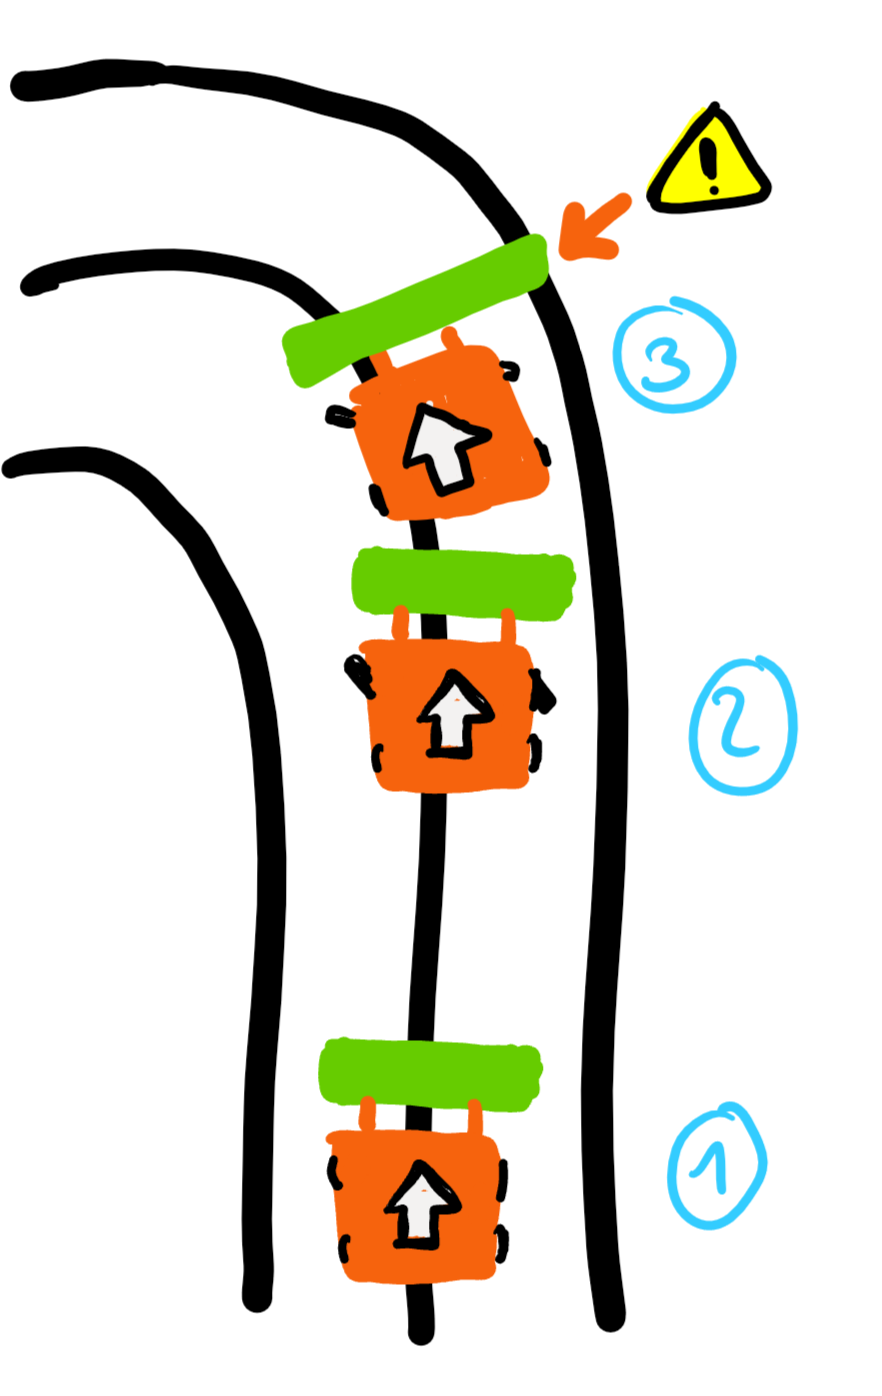
\includegraphics[scale=0.5]{img/Sensor/Auto2.png}
		\caption{Die Problematik mit der Streckenbegrenzung.}
	\end{figure}

	
	Das ist ein Phänomen, was in echt sehr häufig passiert. Das Auto versucht dann, am Rand entlang zu fahren und kommt vom Weg ab. 
	
	Die Lösung, die ich mir überlegt habe lautet wie folgt: Man schaut, wie weit der aktuelle Mittelpunkt der Linie $m_{\text{aktuell}} = m_t\in\{1,...,16\}$ von dem Wert eine Messung zuvor $m_{t-1}$ abweicht. Ist $|m_t - m_{t-1}| < 5$, dann macht das bei einer besonders scharfen Kurve noch Sinn. Das könnte z.B. von Punkt (1) zu Punkt (2) in der Abbildung der Fall sein. Ist aber $|m_t - m_{t-1}| \geq 5$, dann weiß man, da ist etwas schief gelaufen, da soll besser der alte Wert $m_{t-1}$ weiter als Mitte verwendet werden. Also $m_{t}$ überschreiben mit $m_{t-1}$. Dadurch kann das Auto auch in scharfe Kurven fahren. Hier wäre als noch bessere Lösung wieder ein PID Regler eine weitere Option, die aus Zeitgründen nicht genutzt wurde.
	
	\subsubsection{Weitere Funktionalität: Das erkennen von doppelten Quer-Linien}
	Ein weiteres Feature, was ich programmieren wollte, ist die Erkennung von doppelten Querlinien, mit denen das Auto besondere Infos bekommt. Querlinien sind orthogonal zur eigentlichen Fahrbahn verlaufende Linien. Sie treten doppelt hintereinander in kurzen Abständen auf. Dabei soll das Auto auch erkennen, ob die doppelte Querlinie rechts, links oder auf beiden Seiten ist. Dieses Feature funktioniert nur bedingt und unzuverlässig. Etwa in 70\% der Fälle, und es wurden bessere Ergebnisse erzielt, wenn das Auto per USB Kabel mit dem Laptop verbunden und gleichzeitig der Stromschalter umlegt war. Es wird dringend darauf hingewiesen, dazu das Stomversorgungskabel von den Batterien zum ESP32 herauszuziehen, da sonst die Spannung der Batterien am USB Port vom Laptop hängt, was das Gerät zerstören kann. Bislang wurde nur die Ausgabe auf der Konsole eingerichtet: Ein R für zwei Querstreifen rechts, ein L für links und ein G für zwei durchgezogene Querstreifen.
	
	\begin{figure}[H]
		\centering
		\label{sensor9}
		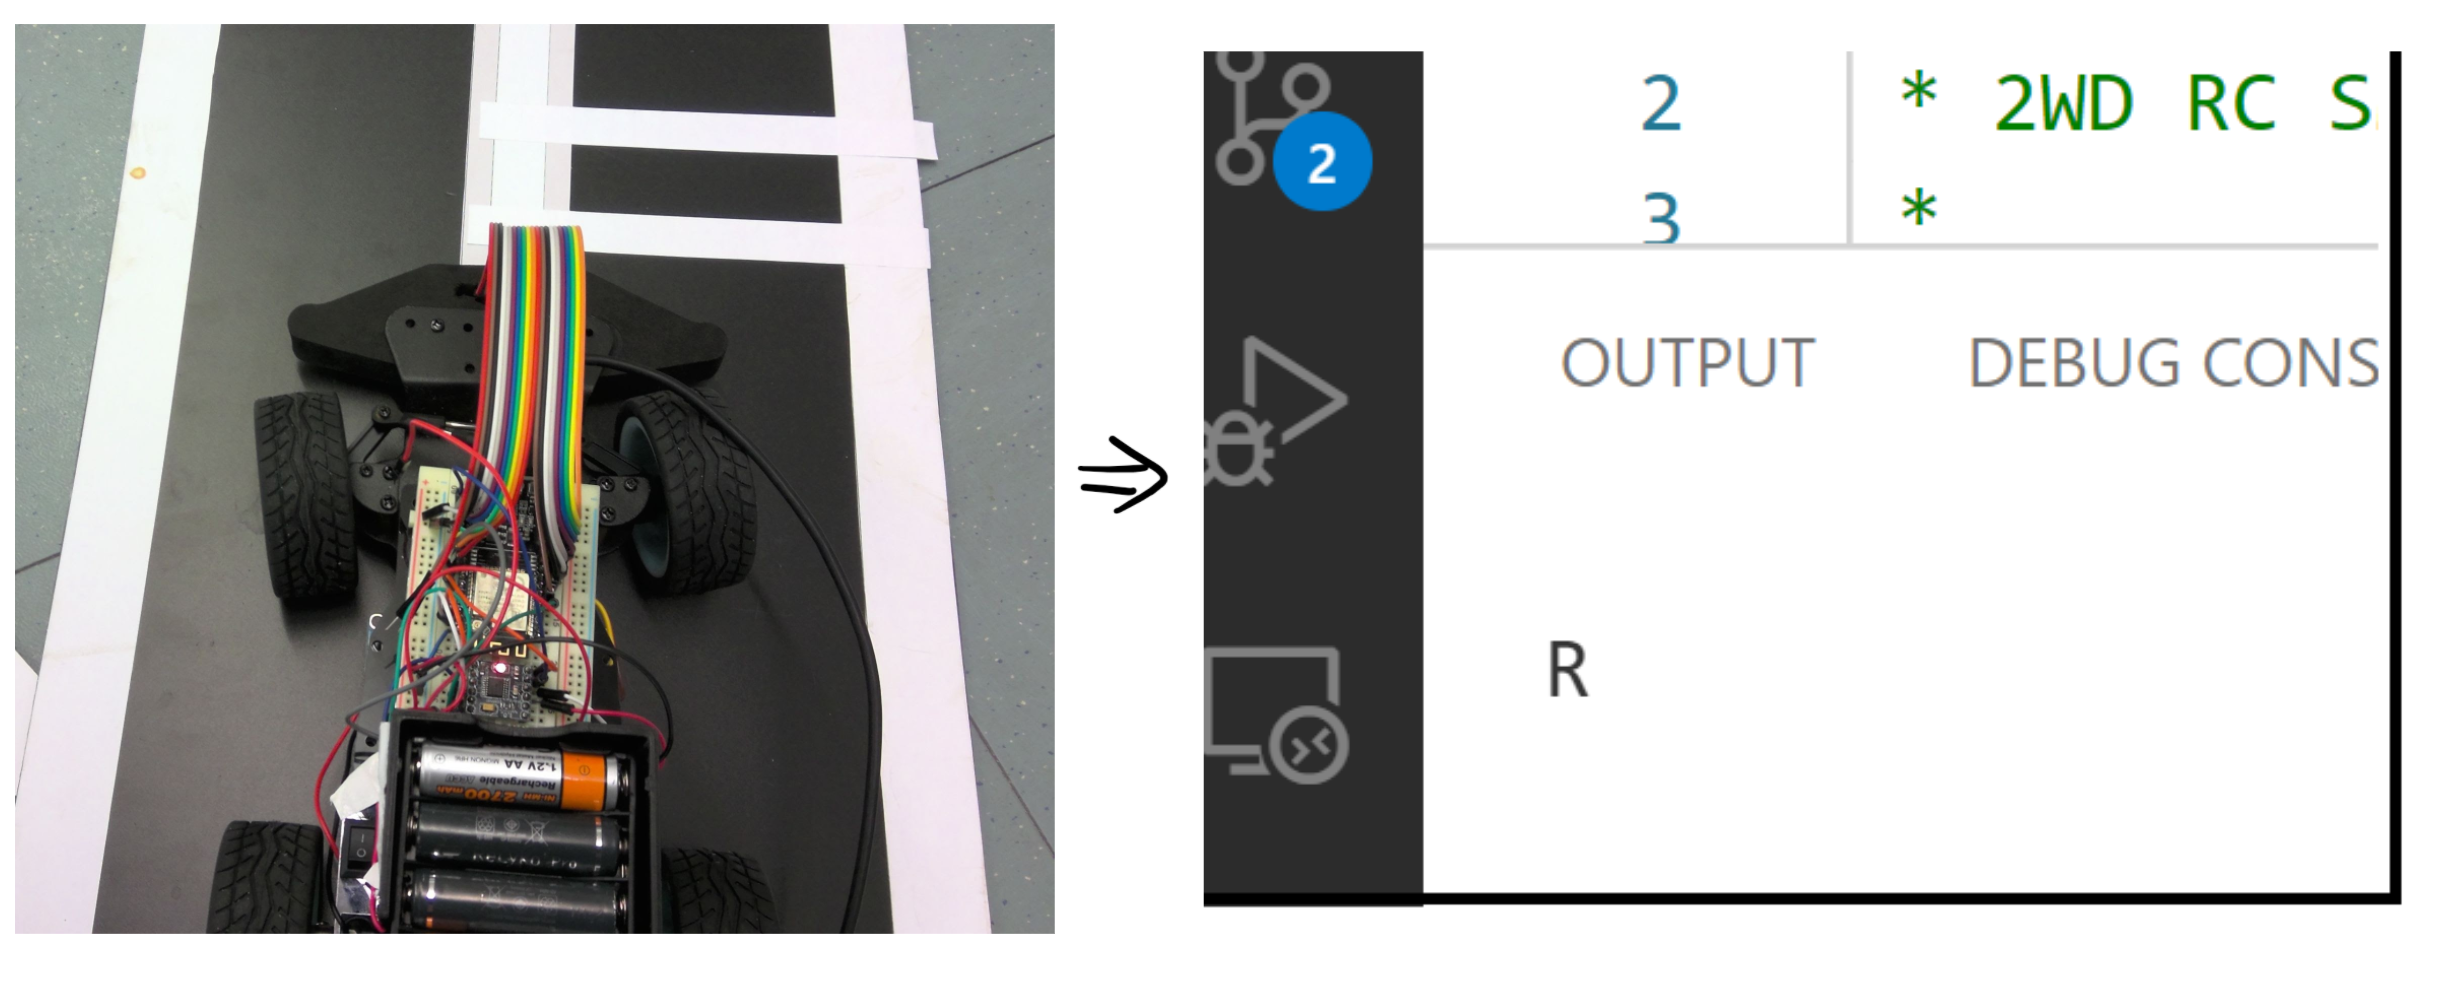
\includegraphics[scale=0.55]{img/Sensor/Sensor9.png}
		\caption{Erkennen der Querlinien.}
	\end{figure}

	
	Wie erwähnt ist das Feature noch nicht ausgereift. Und noch ein Hinweis: Die Erkennung funktioniert nur wenn zwei Querstreifen in kurzem Abstand hintereinander folgen. Es reicht also nicht bloß ein einzelner Querstreifen. Das wurde absichtlich so umgesetzt.
	
	%\subsubsection{PID Regler}
	
	\subsection{Interface}
	
        Um den Overhead so gering wie möglich zu halten, haben wir uns entschieden, die Kommunikation mit unseren Methoden nach außen binär darzustellen. Das Interface findet man in der Datei src/vehicleInterface.
        Zuerst etwas zu den Operatoren, die zur Verwaltung dieser 5 Bytes. Wir verwenden den Shift Operator nach links. 
        Dabei wird eine binäre Zahl n Bits nach links verschoben z.B. 0001 (1) shift 3 = 1000 (8). Da wurde die 1 3 Stellen nach links verschoben. Ein anderes Beispiel 0011 (3) shift 2 = 1100 (12).
        Dafür brauchen wir insgesamt 5 Bytes (40 Bits), wobei wir bei dem ersten Byte nur 3 Bits brauchen. 
        00000000 00000000 00000000 00000000 00000000 
        (1)	     (2)      (3)      (4)      (5)
        
        \begin{itemize}
            \item (1): Das erste Byte ist für die Spurinformationen zuständig. Das erste Bit von links ist auf 1 gesetzt, wenn ein Spurwechsel stattfinden soll. Das zweite Bit ist auf 1 gesetzt, wenn eine 90 Grad Kurve kommt. Das dritte Bit ist auf 1 gesetzt, wenn der kommende Spurwechsel nach rechts ausfällt, andernfalls ist es 0. Wie oben erwähnt wurde, sind hier 5 Bits frei.
            \item (2): Das zweite Byte ist für den Drehwinkel zuständig. Dabei dient das höchste Bit als dem Vorzeichen. Wie in \autoref{Lenkung} erwähnt, ist der Winkel -35 bis 35.
            Die restlichen 7 Bits sind dann für den eigentlichen Wert ohne das Vorzeichen. 
            Beispiel: 1000 1100 = -12, 0001 0011 = 19
            \item (3): Das dritte Byte ist für die Geschwindigkeit zuständig. Die maximale Geschwindigkeit beträgt 255, von daher sind 8 Bits ausreichen.
            \item (4) und (5): Die Bytes 4 und 5 sind für die Sensoren zuständig. (siehe \autoref{Sensorik})
        \end{itemize}
        
        In der Datei vehicleInterface werden Macros verwendet, um den Shift-Operator auszuführen.
        Bei dem ersten Byte wird also eine Eins 7 Bits nach links verschoben, dann ist das erste Bit auf 1 gesetzt und man hat dann die Informationen, dass ein Spurwechsel stattfinden soll.
        Wir bieten dem Benutzer 5 Methoden zur Verwaltung des Fahrzeuges an:
        
        \begin{itemize}
            \item getLaneInfos(linechange, rightangle, rlcurve):
            Die Methode nimmt 3 Werte entgegen.
            \begin{itemize}
                \item Linechange: ‘Y‘ oder ‘N‘
                \item Rightangle: ‘Y‘ oder ‘N‘
                \item rlcurve: ‘R’ oder ‘L‘
            \end{itemize}
            
            und gibt 8 Bits zurück, die entsprechend den entgegengenommenen Werten gesetzt sind.
            \item getSpeed(speed):
            Nimmt einen Wert entgegen und gibt diesen als 8 Bits zurück.
            \item getAngle(angle):
            Nimmt einen Wert entgegen und gibt diesen als 8 Bits zurück, bei denen das erste Bit von links auf eins gesetzt ist, falls der entgegengenommene Wert negativ ist, und die restlichen 7 Bits sind dann der Wert ohne das Vorzeichen.
            \item getSensors(sensors):
            Nimmt einen Wert entgegen und gibt diesen zurück.
            \item translateValues(interface):
            Die Methode nimmt einen Wert (16 Bits) entgegen und führt die entsprechenden Funktionen aus (driveforward, turnsurvo).
            Der entgegengenommene Wert wird in 2 Werte (jeweils 8 Bits) geteilt. 
            \begin{itemize}
                \item Die ersten 8 Bits steuern den Lenkwinkel. Dabei wird der Wert Interface mit dem Operator 'and' mit  255 = 00000000 11111111 verundet, dadurch erhält man die letzten 8 Bits.
                \item Die letzten 8 Bits sind für die Geschwindigkeit zuständig. Die bekommt man, indem man der Wert vom Interface mit Operator ‘and‘ mit 11111111 00000000 verundet.
            \end{itemize}
            Die jeweiligen Funktionen werden dann mit den jeweiligen Werten ausgeführt.
        \end{itemize}
    
    	Das Steuern des Fahrzeug ist somit durch aufrufen der Methoden controlVehicleSerial , oder controlVehicleManual mit der Geschwindigkeit und Lenkwinkel als Parameter, nötig. Den Zustand kann man über die Methode refreshInformations abfragen. Der Abschliessende Schritt, das Aufrufen dieser Methoden mit entsprechenden Parametern, ist noch nicht Implementiert.
    	
    	\section{Fazit}
    	
    	Alles in allem konnten wir einen großen Anteil der Ziele durchsetzten. Die Möglichkeit, alle Komponenten der Steuerung, zu kontrollieren und das Auslesen des Sensors dienen als Basis für das erfolgreiche Fahren auf einer simplen, ovalen Strecke und das erkennen der Markierungen für Lane-Switches und 90° Kurven. Durch zu großen Focus auf das Fahren ist es uns leider nicht gelungen, das Interface in den ersten 2 Wochen fertig zu stellen. Ein paar Änderungen wurden noch nachträglich gemacht. Dadurch war es uns leider nicht mehr möglich, die Kontrolle des Fahrzeuges durch das Interface zu testen.
    	 
